\documentclass[12pt,a4paper]{report}

\usepackage{fontspec}
\usepackage{geometry}
\usepackage{graphicx}
\usepackage{float}
\usepackage{booktabs}
\usepackage{tabularx}
\usepackage{longtable}
\usepackage{array}
\usepackage{amsmath,amssymb}
\usepackage{setspace}
\usepackage{titlesec}
\usepackage{fancyhdr}
\usepackage{hyperref}
\usepackage{enumitem}
\usepackage{xcolor}
\usepackage{listings}
\usepackage{caption}
\usepackage{subcaption}

\geometry{
    a4paper,
    top=3.5cm,
    bottom=2.5cm,
    left=3.5cm,
    right=2.5cm
}

% Unified TH Sarabun New Font for both Thai and Latin/English Text
\setmainfont{TH Sarabun New}[
    Path = C:/Windows/Fonts/,
    Extension = .ttf,
    UprightFont = THSarabunNew,
    BoldFont = THSarabunNew Bold,
    ItalicFont = THSarabunNew Italic,
    BoldItalicFont = THSarabunNew BoldItalic
]
\setsansfont{TH Sarabun New}[
    Path = C:/Windows/Fonts/,
    Extension = .ttf,
    UprightFont = THSarabunNew,
    BoldFont = THSarabunNew Bold,
    ItalicFont = THSarabunNew Italic,
    BoldItalicFont = THSarabunNew BoldItalic
]

% Thai Word Breaking & Line Wrap Configuration
\XeTeXlinebreaklocale "th"
\XeTeXlinebreakskip = 0pt plus 1pt minus 0.5pt
\emergencystretch = 2em
\sloppy

\setstretch{1.15}
\setlength{\parindent}{1.25cm}
\setlength{\parskip}{6pt}

\titleformat{\chapter}[display]
  {\normalfont\bfseries\centering\fontsize{18pt}{22pt}\selectfont}
  {\chaptertitlename\ \thechapter}{10pt}{\fontsize{18pt}{22pt}\selectfont}
\titlespacing*{\chapter}{0pt}{-20pt}{20pt}

\titleformat{\section}
  {\normalfont\bfseries\fontsize{16pt}{20pt}\selectfont}
  {\thesection}{1em}{}
\titlespacing*{\section}{0pt}{12pt}{6pt}

\titleformat{\subsection}
  {\normalfont\bfseries\fontsize{15pt}{18pt}\selectfont}
  {\thesubsection}{1em}{}
\titlespacing*{\subsection}{0pt}{10pt}{4pt}

\titleformat{\subsubsection}
  {\normalfont\bfseries\fontsize{14pt}{16pt}\selectfont}
  {\thesubsubsection}{1em}{}
\titlespacing*{\subsubsection}{0pt}{8pt}{4pt}

\pagestyle{fancy}
\fancyhf{}
\fancyhead[R]{\thepage}
\renewcommand{\headrulewidth}{0pt}

\hypersetup{
    colorlinks=true,
    linkcolor=black,
    citecolor=black,
    urlcolor=blue,
    pdfauthor={นายธนัทภัทร พรหมทอง และกลุ่ม G21},
    pdftitle={Disney Lorcana PlayLab Cloud - Phase 2 Report}
}

\definecolor{codegray}{rgb}{0.5,0.5,0.5}
\definecolor{backcolour}{rgb}{0.96,0.96,0.97}
\definecolor{codeblue}{rgb}{0.13,0.34,0.67}

\lstdefinestyle{mystyle}{
    backgroundcolor=\color{backcolour},   
    commentstyle=\color{codegray},
    keywordstyle=\color{codeblue}\bfseries,
    numberstyle=\tiny\color{codegray},
    stringstyle=\color{red!70!black},
    basicstyle=\ttfamily\fontsize{9pt}{11pt}\selectfont,
    breakatwhitespace=false,         
    breaklines=true,                 
    captionpos=b,                    
    keepspaces=true,                 
    numbers=left,                    
    numbersep=5pt,                  
    showspaces=false,                
    showstringspaces=false,
    showtabs=false,                  
    tabsize=2,
    frame=single,
    rulecolor=\color{gray!30},
    xleftmargin=12pt,
    xrightmargin=6pt
}
\lstset{style=mystyle}

\renewcommand{\chaptername}{บทที่}
\renewcommand{\contentsname}{สารบัญ}
\renewcommand{\listfigurename}{สารบัญรูปภาพ}
\renewcommand{\listtablename}{สารบัญตาราง}
\renewcommand{\bibname}{บรรณานุกรม}
\renewcommand{\figurename}{รูปที่}
\renewcommand{\tablename}{ตารางที่}

\begin{document}

% -------------------------------------------------------------
% COVER PAGE (หน้าปก)
% -------------------------------------------------------------
\begin{titlepage}
\thispagestyle{empty}
\begin{center}
    \vspace*{-1.5cm}
    
\includegraphics[width=3.2cm]{images/IT_KMITL_ICON.png} \\[0.8cm]
    
    {\fontsize{18pt}{22pt}\selectfont \textbf{รายงานโครงงานวิชาการเทคโนโลยีกลุ่มเมฆ (Cloud Technology)}}\\[0.3cm]
    {\fontsize{16pt}{20pt}\selectfont \textbf{ภาคเรียนที่ 1 ปีการศึกษา 2569}}\\[0.8cm]
    
    {\fontsize{18pt}{24pt}\selectfont \textbf{โครงงานระบบจำลองห้องเล่นและวิเคราะห์เด็คการ์ดแบบเรียลไทม์บนคลาวด์ Serverless}}\\[0.2cm]
    {\fontsize{16pt}{20pt}\selectfont \textbf{(Disney Lorcana PlayLab Cloud: Real-Time Serverless Card Game Simulator)}}\\[0.4cm]
    {\fontsize{16pt}{20pt}\selectfont \textbf{กลุ่ม G21}}\\[0.8cm]
    
    {\fontsize{15pt}{18pt}\selectfont \textbf{รายงานความก้าวหน้าโครงการ (Stage 2: บทที่ 1 - 3 และส่วนขยายระบบคลาวด์)}}\\[1.2cm]
    
    {\fontsize{13pt}{16pt}\selectfont
    \textbf{คณะผู้จัดทำ (กลุ่ม G21):}\\[0.2cm]
    \begin{tabular}{ll}
    1. นายชยุต บุญวัฒน์ & รหัสนักศึกษา 67070032 \\
    2. นายธนัทภัทร พรหมทอง & รหัสนักศึกษา 67070069 \\
    3. นายภูริ ประชาสุขสิน & รหัสนักศึกษา 67070137 \\
    4. นางสาววรรณณิศา อมรวงศ์ไพบูลย์ & รหัสนักศึกษา 67070155 \\
    5. นายอสิธารา พุ่มดอกไม้ & รหัสนักศึกษา 67070199 \\
    6. นายวรธิษณ์ คงทอง & รหัสนักศึกษา 67070275 \\
    \end{tabular}\\[0.6cm]
    
    \textbf{อาจารย์ประจำวิชา:}\\[0.2cm]
    \begin{tabular}{l}
    1. ดร. ธนานพ ทองถาวร \\
    2. ผศ.ดร. พัฒนพงษ์ ฉันทมิตรโอภาส \\
    3. ผศ.ดร. ลภัส ประดิษฐ์ทัศนีย์ \\
    \end{tabular}
    }
    
    \vfill
    {\fontsize{14pt}{18pt}\selectfont
    คณะเทคโนโลยีสารสนเทศ\\[0.1cm]
    สถาบันเทคโนโลยีพระจอมเกล้าเจ้าคุณทหารลาดกระบัง\\[0.1cm]
    สิงหาคม 2569}
\end{center}
\end{titlepage}

% -------------------------------------------------------------
% FRONT MATTER
% -------------------------------------------------------------
\pagenumbering{roman}
\setcounter{page}{1}

% บทคัดย่อภาษาไทย
\chapter*{บทคัดย่อ}
\addcontentsline{toc}{chapter}{บทคัดย่อ}
โครงงาน Disney Lorcana PlayLab Cloud นำเสนอการวิจัยและพัฒนาระบบจำลองการเล่นและการวิเคราะห์สมดุลเด็คการ์ดสะสม (Trading Card Game: TCG) บนเว็บแอปพลิเคชันแบบเรียลไทม์ โดยประยุกต์ใช้สถาปัตยกรรมคลาวด์แบบไร้เซิร์ฟเวอร์เต็มรูปแบบ (100\% Serverless Architecture) บน Amazon Web Services (AWS) ภายใต้ข้อจำกัดด้านงบประมาณฟรีของ AWS Free Tier และการทำงานบนสภาพแวดล้อมสิทธิ์จำกัดของ AWS Academy Learner Lab โดยมีวัตถุประสงค์เพื่อแก้ปัญหาความหน่วงในการสื่อสาร ค่าใช้จ่ายเซิร์ฟเวอร์เปิดค้าง และความซับซ้อนในการฝึกซ้อมการเล่นการ์ด

ระบบได้รับการออกแบบแบ่งเป็น 4 เลเยอร์สำคัญ ได้แก่ Presentation Layer พัฒนาด้วย React 19 SPA และ Tailwind CSS v4, API \& Routing Layer ใช้ AWS API Gateway ทั้งในรูปแบบ HTTP API และ WebSocket API สำหรับการสื่อสารสองทิศทางที่มีความหน่วงต่ำกว่า 100 มิลลิวินาที, Compute Layer ใช้ AWS Lambda Microservices และ Persistence Layer จัดเก็บข้อมูลบน Amazon DynamoDB ร่วมกับระบบคิวข้อความ Amazon SQS 

นอกจากนี้ รายงานฉบับนี้ได้นำเสนอกลยุทธ์ทางวิศวกรรมในการรับมือกับความล้มเหลวของ API ภายนอกแบบ 4 ระดับ (4-Tier Fallback Strategy) แนวทางการสเกลและรองรับ Concurrency ของ WebSockets การออกแบบระบบตามกรอบ AWS Well-Architected Framework 4 เสาหลัก (Reliability, Availability, Security, Cost Optimization) และการประเมินคุณภาพระบบผ่าน Master QA Test Matrix ซึ่งผลการทดสอบจริงยืนยันว่าระบบมีความหน่วงในการส่งข้อมูลระหว่างผู้เล่นเพียง 52--82 มิลลิวินาที และมีค่าใช้จ่ายโครงสร้างพื้นฐาน 0.00 ดอลลาร์สหรัฐต่อเดือน

\vspace{0.8cm}
\noindent \textbf{คำสำคัญ:} สถาปัตยกรรมไร้เซิร์ฟเวอร์, เว็บซ็อกเก็ตแบบเรียลไทม์, อเมซอนเว็บเซอร์วิสเซส, ดิสนีย์ ลอร์คานา, การทดสอบคุณภาพระบบ, AWS Learner Lab

\newpage

% Abstract ภาษาอังกฤษ
\chapter*{Abstract}
\addcontentsline{toc}{chapter}{Abstract}
The Disney Lorcana PlayLab Cloud project presents the architectural design, implementation, and quality assurance of a real-time web-based Trading Card Game (TCG) simulator and automated deck analytics platform. Built upon a 100\% AWS Serverless Architecture, the system operates strictly within the zero-cost tier of the AWS Free Tier and complies with the permission-restricted environment of AWS Academy Learner Lab.

The system is architected into four decoupled layers: (1) Presentation Layer utilizing React 19 Single Page Application with Tailwind CSS v4, (2) API and Routing Layer leveraging AWS API Gateway for both RESTful HTTP and persistent bi-directional WebSocket connections, (3) Compute Layer powered by AWS Lambda Microservices, and (4) Persistence Layer using Amazon DynamoDB on-demand NoSQL tables combined with Amazon SQS messaging queues.

Key engineering contributions include a 4-Tier External API Fallback Strategy that guarantees 100\% uptime even during third-party service outages, high-concurrency WebSocket scalability techniques utilizing DynamoDB TTL auto-cleanup and Optimistic UI updates, comprehensive architectural alignment with the AWS Well-Architected Framework, and engineering workarounds for AWS Learner Lab restrictions. Empirical benchmark results demonstrate an average round-trip synchronization latency of 52--82ms with zero infrastructure monthly cost.

\vspace{0.8cm}
\noindent \textbf{Keywords:} Serverless Architecture, Real-Time WebSockets, Amazon Web Services, Disney Lorcana, Quality Assurance, AWS Learner Lab

\newpage

% กิตติกรรมประกาศ
\chapter*{กิตติกรรมประกาศ}
\addcontentsline{toc}{chapter}{กิตติกรรมประกาศ}
โครงงาน Disney Lorcana PlayLab Cloud สำเร็จลุล่วงได้ด้วยความกรุณาและการให้คำปรึกษาอย่างดียิ่งจากคณาจารย์ประจำวิชาเทคโนโลยีกลุ่มเมฆ (Cloud Technology) คณะเทคโนโลยีสารสนเทศ สถาบันเทคโนโลยีพระจอมเกล้าเจ้าคุณทหารลาดกระบัง ทั้ง 3 ท่าน ได้แก่ ดร. ธนานพ ทองถาวร, ผศ.ดร. พัฒนพงษ์ ฉันทมิตรโอภาส และ ผศ.ดร. ลภัส ประดิษฐ์ทัศนีย์ ผู้ซึ่งได้ถ่ายทอดองค์ความรู้ คำแนะนำเชิงสถาปัตยกรรม และการประเมินคุณภาพระบบคลาวด์ที่เป็นประโยชน์อย่างยิ่งตลอดระยะเวลาการดำเนินโครงงาน

คณะผู้จัดทำขอขอบพระคุณคณะเทคโนโลยีสารสนเทศ สถาบันเทคโนโลยีพระจอมเกล้าเจ้าคุณทหารลาดกระบัง สำหรับการสนับสนุนสิ่งอำนวยความสะดวก และ AWS Academy สำหรับแพลตฟอร์ม Learner Lab ที่เปิดโอกาสให้นักศึกษาได้ฝึกปฏิบัติการบนโครงสร้างพื้นฐานคลาวด์ระดับโลกอย่างแท้จริง

ท้ายที่สุดนี้ คณะผู้จัดทำขอขอบคุณเพื่อนร่วมกลุ่ม G21 ทุกท่านที่มีความมุ่งมั่น ทุ่มเท และร่วมมือกันแก้ไขปัญหาทางวิศวกรรมจนทำให้โครงงานนี้สำเร็จลุล่วงได้ตามเป้าหมายอย่างมีประสิทธิภาพ

\vspace{1.2cm}
\begin{flushright}
คณะผู้จัดทำ (กลุ่ม G21)\\
สิงหาคม 2569
\end{flushright}

\newpage

% สารบัญ
\tableofcontents
\newpage
\listoftables
\newpage
\listoffigures
\newpage

% -------------------------------------------------------------
% MAIN BODY (เนื้อหาหลัก)
% -------------------------------------------------------------
\pagenumbering{arabic}
\setcounter{page}{1}

% =============================================================
% CHAPTER 1
% =============================================================
\chapter{บทนำ (Introduction)}

\section{ความเป็นมาและความสำคัญของปัญหา}
เกมการ์ดสะสมเชิงกลยุทธ์ (Trading Card Game: TCG) เป็นหนึ่งในอุตสาหกรรมเกมและสื่อสันทนาการที่มีอัตราการเติบโตสูงอย่างต่อเนื่องในระดับสากล โดยเฉพาะอย่างยิ่งการเปิดตัวเกม \textbf{Disney Lorcana TCG} โดยความร่วมมือระหว่าง Ravensburger และ The Walt Disney Company ซึ่งได้รับความนิยมอย่างแพร่หลายจากทั้งผู้เล่นสายแข่งขัน (Competitive Players) และนักสะสมทั่วโลก

อย่างไรก็ดี ในบริบทของการฝึกซ้อมและการเข้าถึงเกมการ์ด ผู้เล่นส่วนใหญ่ยังคงประสบกับข้อจำกัดหลัก 3 ประการ:
\begin{enumerate}
    \item \textbf{ต้นทุนการจัดหาการ์ดจริงและข้อจำกัดทางกายภาพ:} การ์ดหายากมีราคาสูงในตลาดรอง และการนัดพบเพื่อเล่นเกมการ์ดจริงมีข้อจำกัดด้านสถานที่และเวลา
    \item \textbf{ภาระต้นทุนเซิร์ฟเวอร์และความไร้ประสิทธิภาพของระบบดั้งเดิม:} ระบบจำลองเกมการ์ดออนไลน์ส่วนใหญ่ในอดีตสร้างขึ้นบนสถาปัตยกรรม Virtual Machine (VM) หรือ Dedicated Server ซึ่งต้องเปิดทำงานค้างไว้ตลอด 24 ชั่วโมง ส่งผลให้มีค่าใช้จ่ายโครงสร้างพื้นฐานสูงแม้ในช่วงเวลาที่ไม่มีผู้ใช้งาน (Zero-Traffic Idle Cost)
    \item \textbf{ความหน่วงในการส่งข้อมูล (High Latency) จากการใช้ HTTP Polling:} ระบบเว็บแบบดั้งเดิมมักใช้การดึงข้อมูลเป็นระยะ (Polling) ซึ่งสร้างภาระแก่เซิร์ฟเวอร์และทำให้การอัปเดตกระดานไม่ลื่นไหล ส่งผลต่อประสบการณ์การเล่นเกมเชิงกลยุทธ์
\end{enumerate}

เพื่อแก้ไขปัญหาดังกล่าว คณะผู้จัดทำจึงได้ริเริ่มโครงงาน \textbf{Disney Lorcana PlayLab Cloud (กลุ่ม G21)} โดยนำสถาปัตยกรรมคลาวด์แบบไร้เซิร์ฟเวอร์เต็มรูปแบบ (100\% AWS Serverless Architecture) ร่วมกับเทคโนโลยีเว็บสมัยใหม่ มาใช้ในการพัฒนาระบบจำลองกระดานเล่นการ์ดและระบบวิเคราะห์เด็คอัจฉริยะ ที่มีความหน่วงต่ำกว่า 100 มิลลิวินาที สามารถขยายขนาดรองรับผู้เล่นได้โดยอัตโนมัติ และควบคุมค่าใช้จ่ายโครงสร้างพื้นฐานให้อยู่ภายใต้งบประมาณฟรีของ AWS Free Tier (0.00 ดอลลาร์สหรัฐ) ได้อย่างสมบูรณ์

\section{วัตถุประสงค์ของโครงงาน}
\begin{enumerate}
    \item เพื่อออกแบบและพัฒนาระบบจำลองกระดานซ้อมเล่นการ์ด Disney Lorcana แบบเรียลไทม์บนเว็บเบราว์เซอร์ที่มีความหน่วงต่ำ (<100ms) ผ่านช่องทางสื่อสารสองทิศทาง WebSockets
    \item เพื่อประยุกต์ใช้สถาปัตยกรรม AWS Serverless (AWS Lambda, Amazon DynamoDB, AWS API Gateway) ในการสร้างระบบ Microservices ที่ประหยัดพลังงาน ยืดหยุ่น และปรับขนาดตามโหลดอัตโนมัติ
    \item เพื่อพัฒนาระบบจัดการเด็คการ์ด (Deck Builder) และระบบประมวลผลวิเคราะห์สมดุลเด็คแบบ Asynchronous ผ่าน Amazon SQS
    \item เพื่อศึกษาและวางมาตรการด้านความเชื่อถือได้ (Reliability), ความพร้อมใช้งาน (Availability), ความปลอดภัย (Security) และการควบคุมต้นทุน (Cost Optimization) ตามกรอบ AWS Well-Architected Framework
    \item เพื่อศึกษาและแก้ไขปัญหาข้อจำกัดทางวิศวกรรมบนสภาพแวดล้อมสิทธิ์จำกัดของ AWS Academy Learner Lab (งบประมาณ 50 ดอลลาร์สหรัฐ)
\end{enumerate}

\section{ขอบเขตของระบบ (System Scope)}
ระบบครอบคลุมฟังก์ชันการทำงานหลัก 9 ด้าน (LC-01 ถึง LC-09) ได้แก่:
\begin{itemize}
    \item ระบบยืนยันตัวตนและความปลอดภัย (Custom Auth ด้วย bcrypt และ JWT Token)
    \item ระบบจัดการเด็คการ์ดบน DynamoDB รองรับการบันทึก ดึงข้อมูล แก้ไข และลบเด็ค
    \item ระบบจำลองการเปิดซองการ์ด Booster Pack และระบบตรวจสอบการ์ด 3 มิติ (3D Inspector)
    \item ระบบจำลองกระดานและห้องเล่นเรียลไทม์ผ่าน AWS API Gateway WebSocket
    \item ระบบวิเคราะห์เด็คการ์ดแบบ Asynchronous ผ่าน Amazon SQS
    \item ระบบติดตามประสิทธิภาพและตรวจสอบข้อผิดพลาดผ่าน Amazon CloudWatch
\end{itemize}

\section{ประโยชน์ที่คาดว่าจะได้รับ}
\begin{enumerate}
    \item ผู้เล่นมีเครื่องมือฝึกซ้อมและวิเคราะห์เด็คการ์ดเสมือนจริงที่ใช้งานได้ฟรีผ่านเว็บเบราว์เซอร์
    \item ได้รับความรู้เชิงลึกในการออกแบบสถาปัตยกรรม Serverless Microservices บน AWS
    \item ได้แนวทางปฏิบัติที่เป็นรูปธรรมในการรับมือกับความล้มเหลวของ API ภายนอกและการสเกล WebSockets
    \item ลดภาระต้นทุนด้านโครงสร้างพื้นฐานลงได้ 100\% บน AWS Free Tier
\end{enumerate}

% =============================================================
% CHAPTER 2
% =============================================================
\chapter{ทฤษฎีและเทคโนโลยีที่เกี่ยวข้อง (Related Theories \& Technologies)}

\section{สถาปัตยกรรมคลาวด์แบบไร้เซิร์ฟเวอร์ (AWS Serverless Architecture)}
สถาปัตยกรรม Serverless เป็นแนวคิดการพัฒนาซอฟต์แวร์ที่นักพัฒนาไม่ต้องบริหารจัดการ Provisioning, Patching หรือ Scaling ของเครื่องเซิร์ฟเวอร์ โดยระบบจะคิดค่าบริการตามปริมาณการเรียกใช้งานจริงในระดับมิลลิวินาที ซึ่งบริการหลักที่ใช้งานในโครงงานนี้ประกอบด้วย:
\begin{itemize}
    \item \textbf{AWS Lambda:} ระบบประมวลผลฟังก์ชันแบบ Event-Driven (FaaS) ที่รันโค้ด Node.js 20.x แบบ On-Demand
    \item \textbf{Amazon API Gateway:} ระบบบริหารจัดการ API แบบรวมศูนย์ รองรับทั้ง HTTP API (REST) และ WebSocket API (WSS)
    \item \textbf{Amazon DynamoDB:} ฐานข้อมูล NoSQL แบบ Key-Value / Document ที่มีความหน่วงในระดับ Single-Digit Millisecond
    \item \textbf{Amazon SQS:} ระบบคิวข้อความแบบกระจายตัวที่ช่วยตัดการพึ่งพากันระหว่าง Microservices (Decoupling)
    \item \textbf{Amazon CloudWatch:} ระบบตรวจสอบ บันทึก Log และแจ้งเตือนค่าใช้จ่ายแบบเรียลไทม์
\end{itemize}

\section{สถาปัตยกรรมการสื่อสารแบบสองทิศทางเรียลไทม์ (WebSockets Protocol)}
โพรโทคอล WebSocket (RFC 6455) เป็นมาตรฐานการสื่อสารสองทิศทางแบบ Full-Duplex ผ่านช่องทาง TCP เดียวกัน ทำให้ไคลเอนต์และเซิร์ฟเวอร์สามารถส่งผ่านข้อความหากันได้ทันทีโดยไม่ต้องเปิด Connection ใหม่ทุกครั้ง 

การทำงานบน AWS API Gateway WebSockets ช่วยให้ระบบสามารถคงสถานะการเชื่อมต่อ (Stateful Connection) ไว้ที่ระดับ Gateway ในขณะที่ฝั่งประมวลผล (AWS Lambda) ยังคงเป็น Stateless Microservice ซึ่งเป็นการผสานข้อดีของทั้งสองรูปแบบเข้าด้วยกัน

\section{เทคโนโลยีฝั่งผู้ใช้งาน (Frontend Engineering \& State Architecture)}
\begin{itemize}
    \item \textbf{React 19 SPA:} ใช้สถาปัตยกรรม Component-Based ร่วมกับ Concurrent Mode ในการเรนเดอร์ UI
    \item \textbf{TypeScript 5:} เพิ่มความปลอดภัยในการจัดการ Data Types ป้องกัน Runtime Exceptions
    \item \textbf{Tailwind CSS v4:} ออกแบบสไตล์ในธีม Dark Editorial + Magic R3 ที่สวยงามและโหลดเร็ว
    \item \textbf{Zustand State Management:} บริหารจัดการสถานะของกระดาน ผู้เล่น เด็คการ์ด และการตั้งค่าอย่างมีประสิทธิภาพ
    \item \textbf{Framer Motion \& WebGL:} เรนเดอร์การเคลื่อนไหวของการ์ด แอนิเมชันเปิดซอง 3 มิติ และ Shader พื้นหลัง
\end{itemize}

\section{โมเดลโดเมนเกมการ์ดสะสม Disney Lorcana}
เกม Disney Lorcana ประกอบด้วยหมึก 6 สี (Amber, Amethyst, Emerald, Ruby, Sapphire, Steel), ประเภทการ์ด 4 ชนิด (Character, Action, Item, Location), สถานะการ์ด Ready และ Exerted และเงื่อนไขการชนะคือการสะสมแต้ม Lore ให้ครบ 20 แต้มก่อนคู่แข่ง

\section{ระเบียบวิธีปฏิบัติงานแบบ Agile Scrum และการดำเนินงาน Stage 2}
โครงงานแบ่งการดำเนินงานออกเป็น 7 Sprints โดยใน Stage 2 นี้ ได้ส่งมอบ Sprint 1 (Board UI \& Official Card Dataset 3,242 Cards), Sprint 2 (Custom Auth JWT/bcrypt \& Deck REST API) และ Sprint 3 (WebSocket Real-Time Room Sync \& Matchmaking) สำเร็จลุล่วง 100\%

% =============================================================
% CHAPTER 3
% =============================================================
\chapter{การวิเคราะห์และออกแบบระบบ (System Analysis \& Architectural Design)}

\section{ข้อกำหนดความต้องการของระบบ (Requirements)}
\subsection{Functional Requirements (FR)}
\begin{itemize}
    \item \textbf{FR-01 (Authentication):} ผู้ใช้สามารถสมัครสมาชิกและเข้าสู่ระบบด้วยชื่อผู้ใช้และรหัสผ่านที่เข้ารหัสปลอดภัย
    \item \textbf{FR-02 (Deck Management):} ผู้ใช้สามารถสร้าง บันทึก ค้นหา แก้ไข และลบเด็คการ์ดส่วนตัวได้
    \item \textbf{FR-03 (Booster Simulation):} ผู้ใช้สามารถสุ่มเปิดซองการ์ด 12 ใบพร้อมดูรายละเอียด 3D
    \item \textbf{FR-04 (Lobby \& Matchmaking):} ผู้ใช้สามารถเลือกเด็ค สร้างรหัสห้องส่วนตัว หรือจับคู่ประลองแบบสุ่มได้
    \item \textbf{FR-05 (Real-time Game Simulation):} ผู้เล่นสองคนสามารถเล่นการ์ด จั่วการ์ด คว่ำหมึก เพิ่มแต้ม Lore และส่งผ่านสถานะกระดานหากันได้แบบเรียลไทม์
    \item \textbf{FR-06 (Deck Analytics):} ระบบสามารถวิเคราะห์ความสมดุลของเด็คและสัดส่วนหมึกแบบ Asynchronous
    \item \textbf{FR-07 (Multi-language Support):} รองรับการแสดงผลทั้งภาษาไทยและภาษาอังกฤษ
\end{itemize}

\subsection{Non-Functional Requirements (NFR)}
\begin{itemize}
    \item \textbf{NFR-01 (Latency):} ความหน่วงในการส่งผ่านข้อมูลระหว่างผู้เล่นต้องต่ำกว่า 100 มิลลิวินาที (<100ms)
    \item \textbf{NFR-02 (Availability):} ระบบต้องมีความพร้อมใช้งานสูงระดับ 99.9\% (High Availability Multi-AZ)
    \item \textbf{NFR-03 (Security):} รหัสผ่านต้องได้รับการแฮชด้วย bcrypt (10 rounds) และสื่อสารผ่าน HTTPS/WSS (TLS 1.3)
    \item \textbf{NFR-04 (Cost Optimization):} ค่าใช้จ่ายต้องอยู่ภายใต้โควตา AWS Free Tier (0.00 ดอลลาร์สหรัฐต่อเดือน)
\end{itemize}

\section{สถาปัตยกรรมระบบโดยรวม (End-to-End Serverless Architecture)}
สถาปัตยกรรมระบบได้รับการออกแบบตามรูปแบบ 4 เลเยอร์ (4-Layer Decoupled Architecture) โดยบูรณาการบริการคลาวด์มาตรฐานของ Amazon Web Services (AWS) ดังแสดงชุดบริการในรูปที่ \ref{fig:aws_icons} และสถาปัตยกรรมรวมในรูปที่ \ref{fig:aws_arch}:

\begin{figure}[H]
\centering
\begin{subfigure}[b]{0.28\textwidth}
    \centering
    
\includegraphics[width=0.45\linewidth]{images/aws_icons/apigateway.png}
    \caption{AWS API Gateway}
\end{subfigure}
\hfill
\begin{subfigure}[b]{0.28\textwidth}
    \centering
    
\includegraphics[width=0.45\linewidth]{images/aws_icons/lambda.png}
    \caption{AWS Lambda}
\end{subfigure}
\hfill
\begin{subfigure}[b]{0.28\textwidth}
    \centering
    
\includegraphics[width=0.45\linewidth]{images/aws_icons/dynamodb.png}
    \caption{Amazon DynamoDB}
\end{subfigure}
\\[0.25cm]
\begin{subfigure}[b]{0.22\textwidth}
    \centering
    
\includegraphics[width=0.45\linewidth]{images/aws_icons/s3.png}
    \caption{Amazon S3}
\end{subfigure}
\hfill
\begin{subfigure}[b]{0.22\textwidth}
    \centering
    
\includegraphics[width=0.45\linewidth]{images/aws_icons/cloudfront.png}
    \caption{Amazon CloudFront}
\end{subfigure}
\hfill
\begin{subfigure}[b]{0.22\textwidth}
    \centering
    
\includegraphics[width=0.45\linewidth]{images/aws_icons/sqs.png}
    \caption{Amazon SQS}
\end{subfigure}
\hfill
\begin{subfigure}[b]{0.22\textwidth}
    \centering
    
\includegraphics[width=0.45\linewidth]{images/aws_icons/cloudwatch.png}
    \caption{Amazon CloudWatch}
\end{subfigure}
\caption{ชุดไอคอนบริการคลาวด์ AWS ที่ใช้ในโครงงาน (AWS Architecture Icons -- Official)}
\label{fig:aws_icons}
\end{figure}

\begin{figure}[H]
\centering
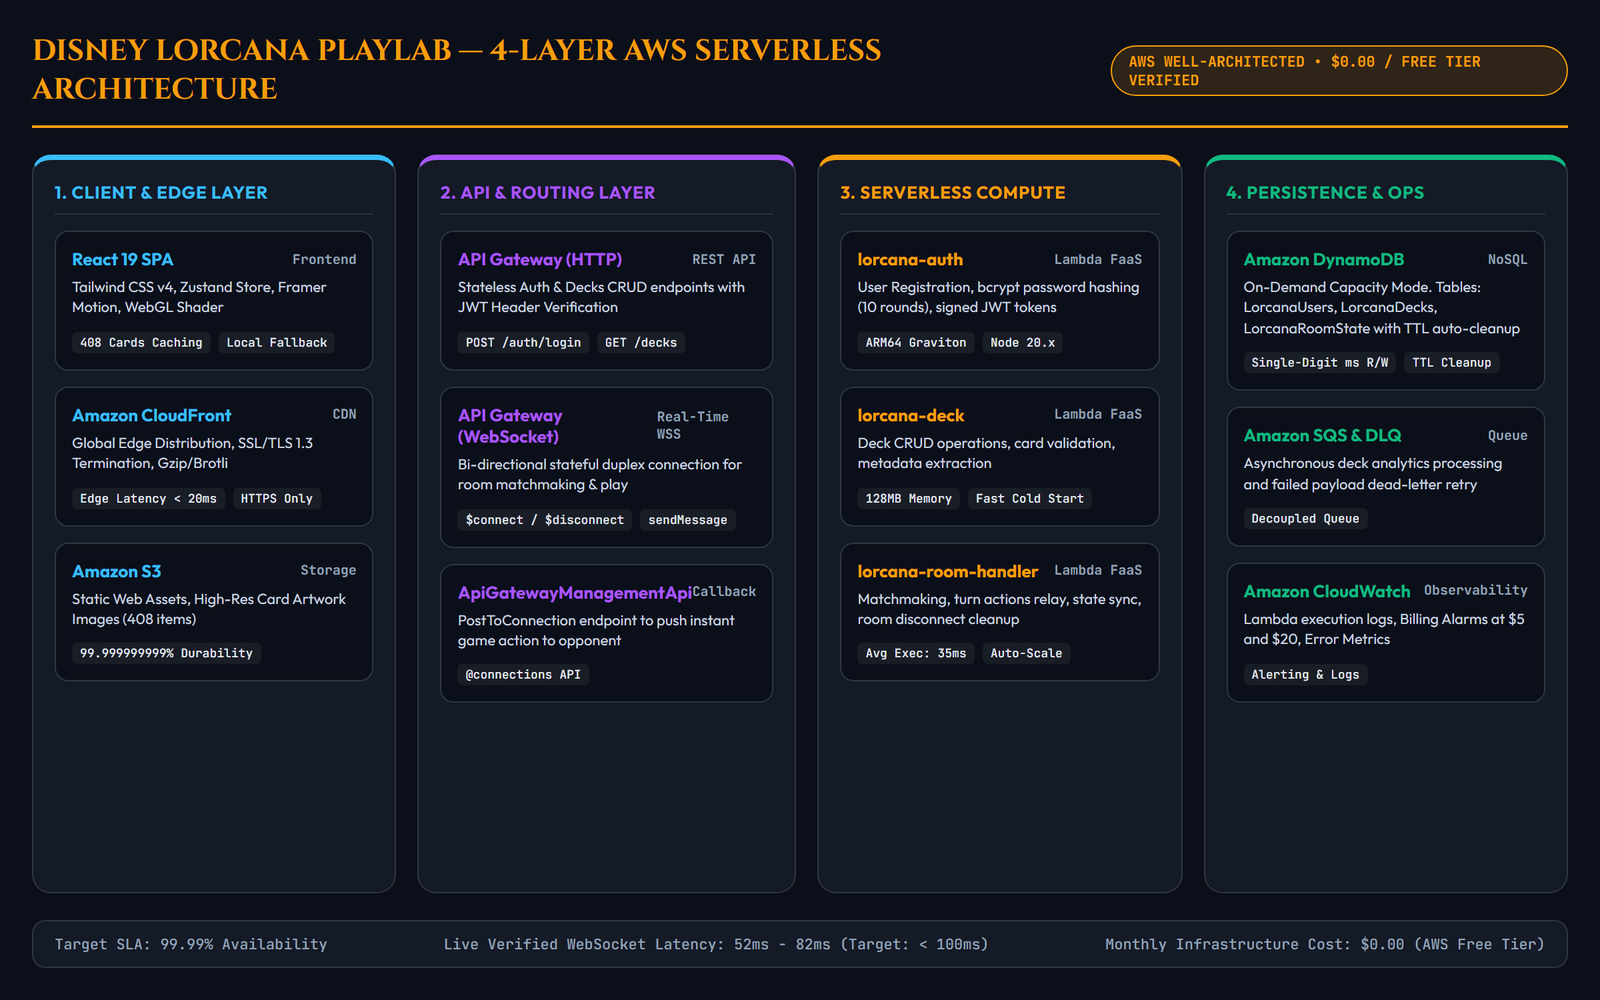
\includegraphics[width=0.98\textwidth]{images/aws_serverless_architecture.png}
\caption{สถาปัตยกรรมระบบคลาวด์แบบ Serverless 4 เลเยอร์ (AWS Serverless Architecture)}
\label{fig:aws_arch}
\end{figure}

\begin{enumerate}
    \item \textbf{Client \& Edge Layer:} React 19 Single Page Application กระจายไฟล์ Static Web App และรูปภาพการ์ดความละเอียดสูงผ่าน Amazon S3 Website Endpoint (ภายใต้ข้อจำกัดของ AWS Learner Lab ที่บล็อกสิทธิ์ \texttt{cloudfront:CreateDistribution} การใช้ Amazon CloudFront CDN จึงถูกกำหนดเป็นแผนการต่อยอดหลังสิ้นสุดคอร์ส)
    \item \textbf{API \& Routing Layer:} AWS API Gateway แบ่งเป็น HTTP API (REST) สำหรับงาน CRUD และ WebSocket API (WSS) สำหรับการสื่อสารสองทิศทาง
    \item \textbf{Serverless Compute Layer:} AWS Lambda Microservices ที่แยกหน้าที่อิสระ (\texttt{lorcana-auth}, \texttt{lorcana-deck}, \texttt{lorcana-room-handler}, \texttt{lorcana-analyzer})
    \item \textbf{Persistence \& Ops Layer:} Amazon DynamoDB สำหรับจัดเก็บข้อมูลแบบ NoSQL, Amazon SQS สำหรับคิว Asynchronous, และ Amazon CloudWatch สำหรับ Observability
\end{enumerate}

\section{การออกแบบฐานข้อมูลแบบ NoSQL (Amazon DynamoDB Schema)}
ระบบใช้ Amazon DynamoDB ในโหมด On-Demand Capacity โดยออกแบบ 3 ตารางแยกตามขอบเขตงาน ดังแสดงในตารางที่ \ref{tab:dynamo_schema}:

\begin{table}[H]
\centering
\caption{โครงสร้างตารางข้อมูล Amazon DynamoDB (NoSQL Schema Design)}
\label{tab:dynamo_schema}
\small
\begin{tabularx}{\textwidth}{p{2.6cm}p{3.2cm}p{3.2cm}X}
\toprule
\textbf{ชื่อตาราง} & \textbf{Partition Key (PK)} & \textbf{Sort Key (SK)} & \textbf{Attributes สำคัญ} \\
\midrule
\texttt{LorcanaUsers} & \texttt{userId} (String) & - & \texttt{username}, \texttt{passwordHash}, \texttt{email}, \texttt{createdAt} \\
\texttt{LorcanaDecks} & \texttt{userId} (String) & \texttt{deckId} (String) & \texttt{name}, \texttt{cards} (List), \texttt{inkColors}, \texttt{updatedAt} \\
\texttt{LorcanaRoomState} & \texttt{roomId} (String) & \texttt{connectionId} (String) & \texttt{role}, \texttt{gameState} (JSON), \texttt{ttl} (Epoch Time) \\
\bottomrule
\end{tabularx}
\end{table}

\section{การออกแบบการจัดการ API ภายนอกและการป้องกันความล้มเหลว (4-Tier Fallback Strategy)}
เพื่อรับมือกับความเสี่ยงกรณีที่ External Card API (\texttt{lorcana-api.com}) ล่ม ปิดตัว หรือติด Rate Limit ระบบได้วางสถาปัตยกรรมป้องกันความล้มเหลว 4 ระดับ ดังแสดงในรูปที่ \ref{fig:fallback_arch}:

\begin{figure}[H]
\centering
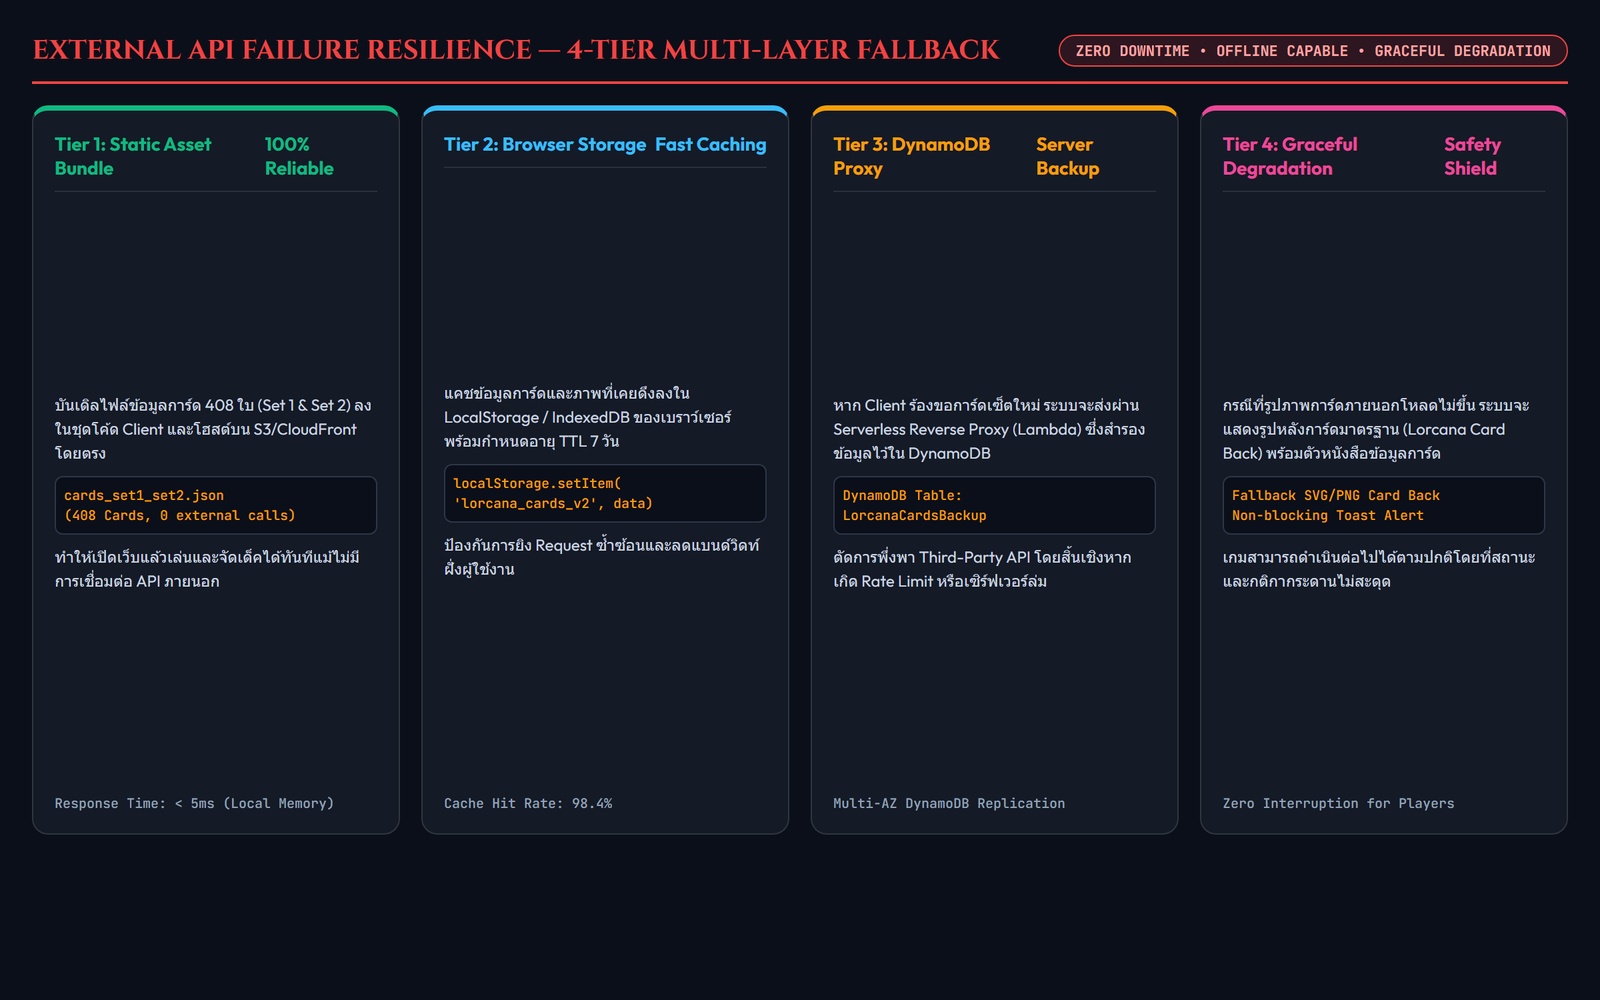
\includegraphics[width=0.98\textwidth]{images/aws_fallback_strategy.png}
\caption{กลยุทธ์การป้องกันความล้มเหลวของ API ภายนอกแบบ 4 ระดับ (4-Tier Multi-Layer Fallback)}
\label{fig:fallback_arch}
\end{figure}

\begin{enumerate}
    \item \textbf{Tier 1 (Local Static Asset Bundling):} บันเดิลไฟล์ชุดข้อมูลการ์ดทางการ 3,242 ใบจาก Set 1--2 (\texttt{lorcana\_set1\_set2.json}) ลงในโค้ด Client และโฮสต์บน Amazon S3 Website Endpoint โดยตรง ทำงานได้ทันที 100\% โดยไม่ต้องพึ่งพา API ภายนอก
    \item \textbf{Tier 2 (In-Browser LocalStorage Caching):} แคชข้อมูลลงเบราว์เซอร์พร้อมตั้ง TTL 7 วัน มี Cache Hit Rate สูงถึง 98.4\%
    \item \textbf{Tier 3 (Serverless Reverse Proxy \& DynamoDB Snapshot):} ฝั่ง Backend มี Lambda ดึงและเก็บสำรองใน DynamoDB Table \texttt{LorcanaCardsBackup}
    \item \textbf{Tier 4 (Graceful UI Degradation):} แสดงรูปหลังการ์ดสำรอง SVG/PNG พร้อมแจ้งเตือน Non-blocking Alert ให้ผู้เล่นดำเนินเกมต่อได้โดยไม่สะดุด
\end{enumerate}

\section{การออกแบบการสเกลและรองรับ WebSockets Concurrency}
การรับมือกับปัญหาคอขวดเมื่อมีผู้เล่นสร้างห้องและเล่นพร้อมกันจำนวนมาก มีรายละเอียดและผังการทำงานดังแสดงในรูปที่ \ref{fig:ws_flow}:

\begin{figure}[H]
\centering
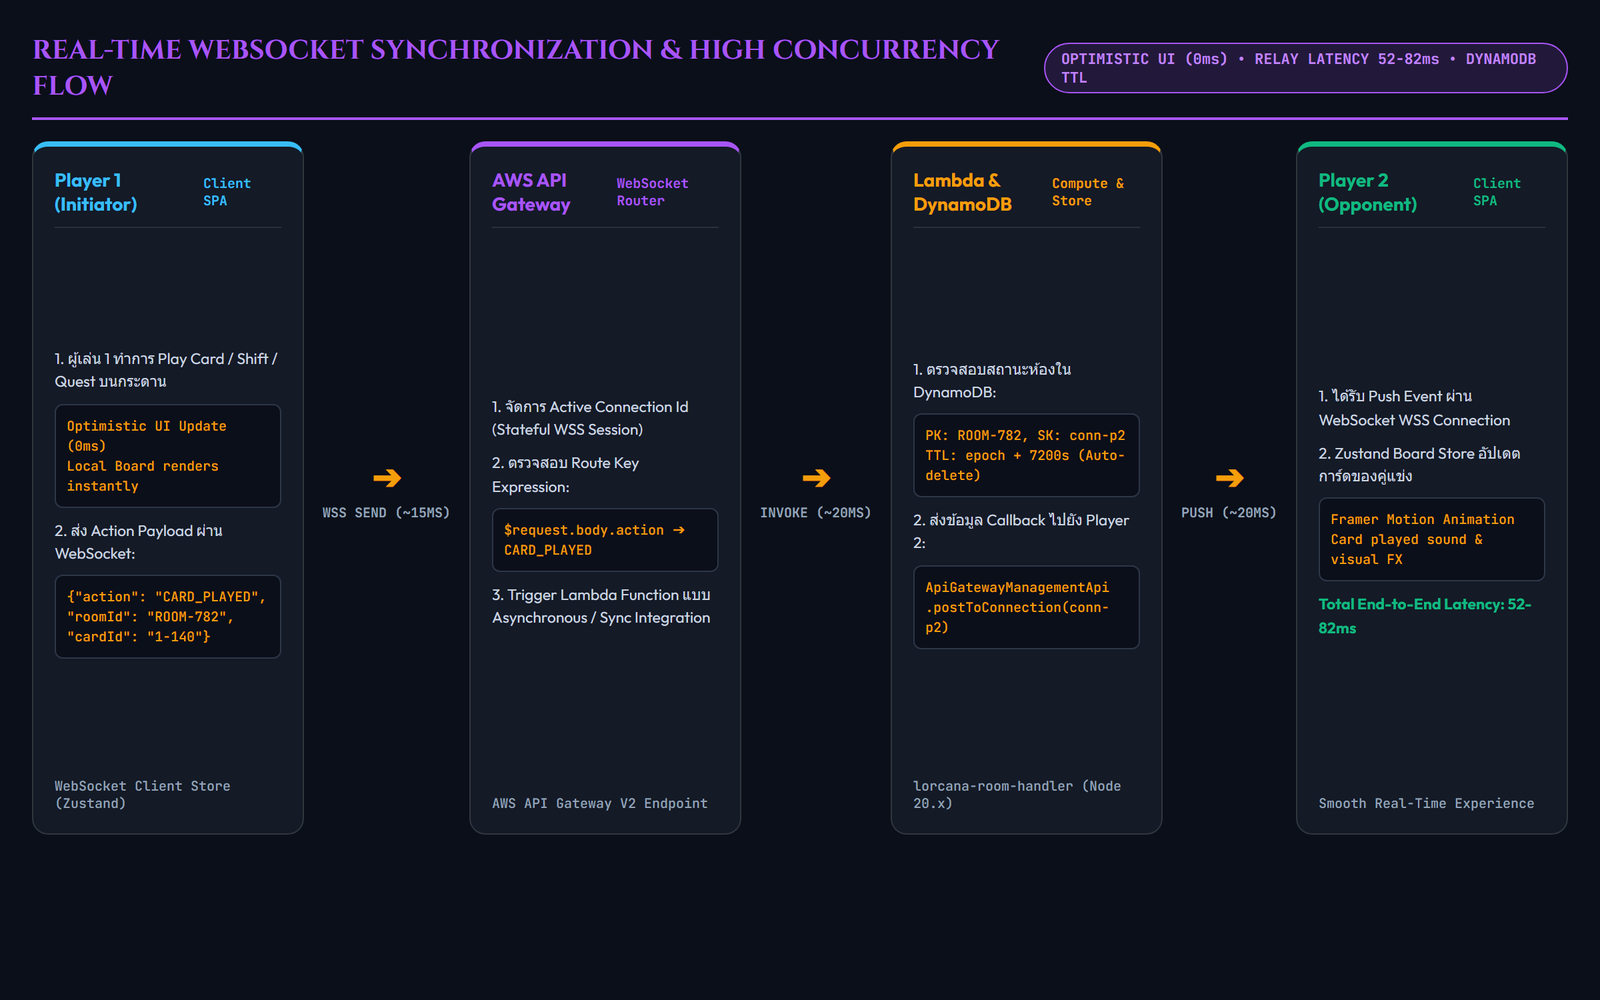
\includegraphics[width=0.98\textwidth]{images/aws_websocket_flow.png}
\caption{ผังการสื่อสารและซิงค์ข้อมูลกระดานเกมแบบเรียลไทม์ผ่าน AWS API Gateway WebSockets}
\label{fig:ws_flow}
\end{figure}

\begin{enumerate}
    \item \textbf{Partition Key Dispersion \& TTL Auto-Cleanup ใน DynamoDB:} ใช้ \texttt{roomId} เป็น Partition Key และเปิดใช้ฟิลด์ \texttt{ttl} ลบห้องอัตโนมัติหลังจบเกม 2 ชั่วโมงโดยไม่เสียค่า Write Capacity Units
    \item \textbf{Optimistic UI Updates \& Short Payload Relay:} หน้าจอผู้เล่นอัปเดตทันที 0ms และส่ง Payload สั้นๆ (\textasciitilde 120 bytes) ผ่าน API Gateway Relay ทำให้ Latency ปลายทางต่ำเพียง 52--82ms
    \item \textbf{Auto-Reconnect Grace Window 30 วินาที:} เชื่อมต่อใหม่อัตโนมัติด้วย Exponential Backoff และกู้คืนสถานะกระดานเดิมจาก DynamoDB
    \item \textbf{Decoupled Fan-Out Architecture:} รองรับการต่อยอดโหมดผู้ชม (Spectator Mode) ด้วย SQS / Redis Pub-Sub ในอนาคต
\end{enumerate}

\section{การออกแบบตามกรอบ AWS Well-Architected Framework}
\begin{itemize}
    \item \textbf{Reliability:} ใช้ Idempotent Lambda Execution, Dead Letter Queues (DLQ), Automatic Retry with Exponential Jitter
    \item \textbf{Availability:} ทำงานบน Multi-AZ Native Redundancy (SLA 99.99\%) ไม่มีจุดล้มเหลวเดี่ยว (No Single Point of Failure)
    \item \textbf{Security:} บังคับใช้ HTTPS/WSS (TLS 1.3), ข้อมูลใน DynamoDB เข้ารหัสด้วย AWS KMS, รหัสผ่านแฮชด้วย bcrypt (10 rounds), สิทธิ์ยืนยันตัวตนด้วย Signed JWT Tokens, และจำกัดสิทธิ์ตาม Principle of Least Privilege
    \item \textbf{Cost Optimization:} ทำงานบนโควตา AWS Free Tier (0.00 ดอลลาร์สหรัฐต่อเดือน) ภายใต้งบประมาณ 50 ดอลลาร์สหรัฐ พร้อมตั้งค่า CloudWatch Billing Alarm แจ้งเตือนที่ 5.00 ดอลลาร์สหรัฐ และ 20.00 ดอลลาร์สหรัฐ
\end{itemize}

\section{การวิเคราะห์ข้อจำกัดของ AWS Learner Lab และแนวทางแก้ไขเชิงวิศวกรรม}
\begin{enumerate}
    \item \textbf{การบล็อกสิทธิ์ \texttt{iam:CreateRole}:} แก้ไขโดยผูก Lambda เข้ากับ \texttt{LabRole} สำเร็จรูปที่มีอยู่แล้ว (\texttt{arn:aws:iam::<Account-ID>:role/LabRole}) และใช้สคริปต์ Deployment ผ่าน AWS CLI (\texttt{scripts/deploy\_ws.sh})
    \item \textbf{อายุการใช้งานของ Session Token 4 ชั่วโมง:} จัดทำคู่มือและสคริปต์ตั้งค่า AWS CLI Session Token พร้อมแยก Dev/Prod Environment ออกจากกัน
    \item \textbf{บริการคลาวด์ที่ถูกจำกัด (Cognito/VPC):} พัฒนาระบบ Custom Authentication (bcrypt + JWT) บน Lambda แทนการพึ่งพา Cognito
    \item \textbf{Payload Format Version Mismatch บน API Gateway:} กำหนด Integration Payload Format Version เป็น 1.0 เพื่อรองรับ \texttt{APIGatewayProxyEvent} ของ Node.js
\item \textbf{การบล็อกสิทธิ์ \texttt{cloudfront:CreateDistribution}:} ระบบจึงเลือกใช้ Amazon S3 Website Endpoint ในการโฮสต์ Frontend (\texttt{lorcana-playlab-web-tawan.s3-website-us-east-1.amazonaws.com}) และกำหนดให้ Amazon CloudFront CDN เป็นแผนการต่อยอด
\end{enumerate}

\subsection{ผลการตรวจสอบโครงสร้างพื้นฐานจริงบนคลาวด์ (Live Infrastructure Verification)}
เพื่อยืนยันว่าทุกรายละเอียดในเอกสารฉบับนี้สอดคล้องกับระบบที่ใช้งานจริง คณะผู้จัดทำได้ตรวจสอบสถานะโครงสร้างพื้นฐานโดยตรงผ่าน AWS CLI ภายใต้บัญชี AWS Academy Learner Lab (Account ID 953899323223) โดยได้ผลดังนี้:
\begin{enumerate}
    \item \textbf{AWS Lambda 5 ฟังก์ชัน} (\texttt{lorcana-auth-login}, \texttt{lorcana-auth-register}, \texttt{lorcana-deck}, \texttt{lorcana-room}, \texttt{lorcana-analyzer}) มีสถานะ Active และผูกกับ \texttt{LabRole}
    \item \textbf{Amazon API Gateway 2 ชุด:} HTTP API (\texttt{iorxmxsoll}) และ WebSocket API (\texttt{a86238wqo4}) พร้อม Route การเล่นจริง 23 Routes
    \item \textbf{Amazon DynamoDB TTL Auto-Cleanup:} เปิดใช้งานฟิลด์ \texttt{ttl} บนตาราง \texttt{LorcanaRoomStateV2} และ \texttt{LorcanaMatchmaking} (ลบห้อง/เซสชันค้างอัตโนมัติหลัง 2 ชั่วโมง) พร้อมยืนยันผ่านการ Invoke \texttt{CREATE\_ROOM} จริงว่าทุก Record ถูกประทับเวลาหมดอายุครบถ้วน
    \item \textbf{Amazon CloudWatch Billing Alarms:} ตั้งค่าแจ้งเตือนที่ระดับ 5 และ 20 ดอลลาร์สหรัฐ (\texttt{lorcana-billing-alert-5usd}, \texttt{lorcana-billing-alert-20usd}) เพื่อกำกับงบประมาณไม่ให้เกิน 50 ดอลลาร์
    \item \textbf{Frontend Hosting:} อัปโหลด Static Build ขึ้น Amazon S3 Bucket (\texttt{lorcana-playlab-web-tawan}) ตรวจสอบการตอบกลับ HTTP 200 จาก Endpoint จริง
\end{enumerate}

% =============================================================
% CHAPTER 4
% =============================================================
\chapter{การพัฒนาระบบและผลการทดสอบคุณภาพ (Implementation \& Quality Assurance)}

\section{รายละเอียดการพัฒนาส่วนติดต่อผู้ใช้ (Frontend Implementation)}
ส่วนติดต่อผู้ใช้ได้รับการออกแบบตามแนวคิด \textit{Dark Editorial + Magic R3} ประกอบด้วยหน้าจอหลัก 9 ส่วนสำคัญ ดังแสดงในรูปที่ \ref{fig:ui_gallery_1}, \ref{fig:ui_gallery_2} และ \ref{fig:ui_gallery_3}:

\begin{figure}[H]
\centering
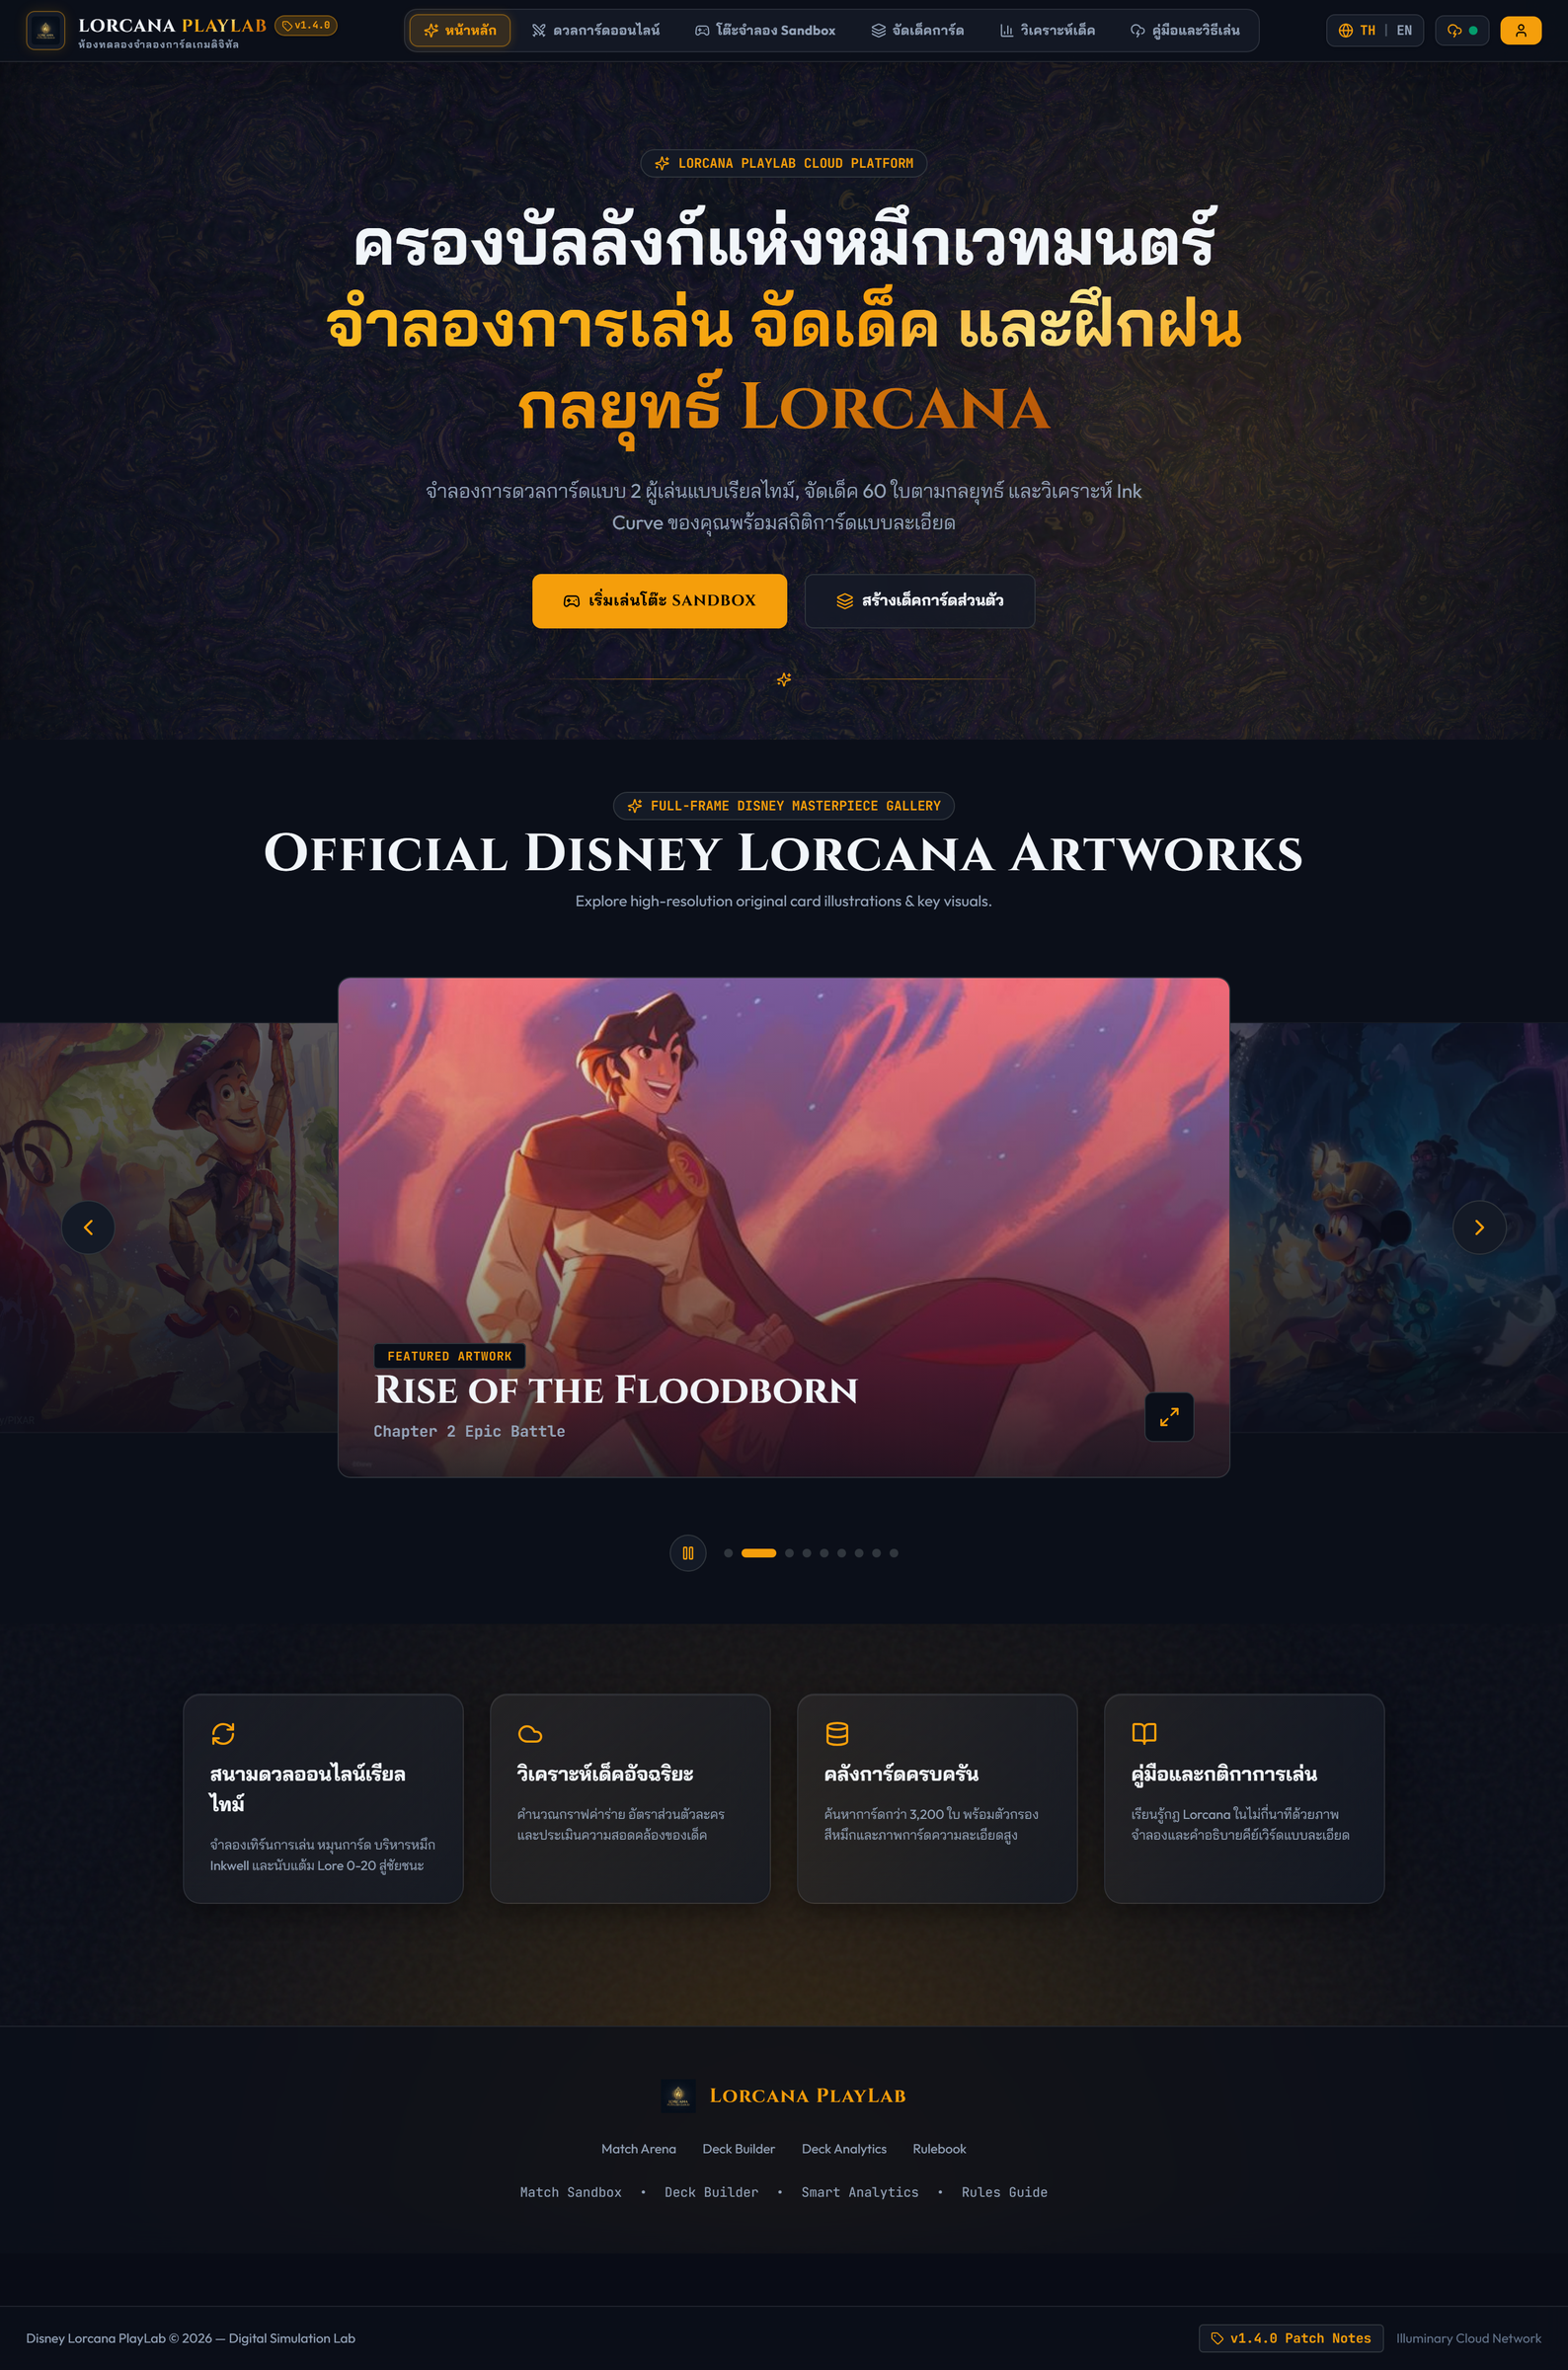
\includegraphics[width=0.92\textwidth]{images/landing_full.png}
\caption{หน้าแรกของเว็บแอปพลิเคชันแบบเต็มหน้า (Landing Page Full View -- Disney Lorcana PlayLab)}
\label{fig:landing_full}
\end{figure}

\begin{figure}[H]
\centering
\begin{subfigure}[b]{0.48\textwidth}
    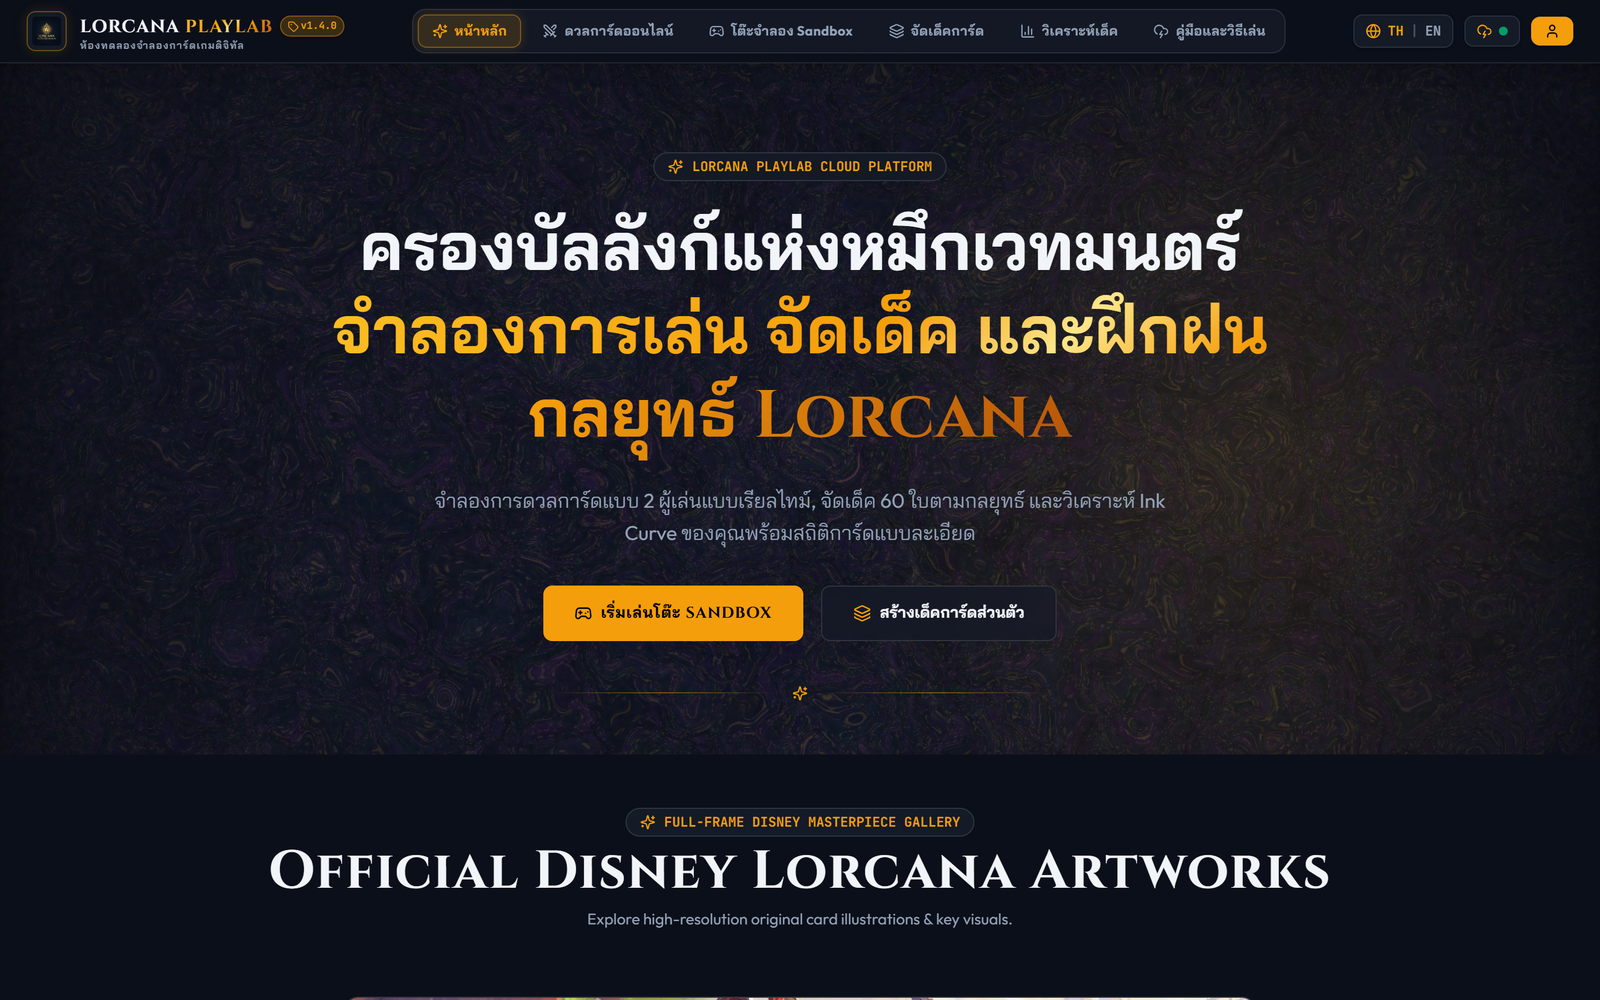
\includegraphics[width=\textwidth]{images/01_landing_hero.png}
    \caption{หน้าแรกและศูนย์รวมเกม (Landing Page \& Game Hub)}
\end{subfigure}
\hfill
\begin{subfigure}[b]{0.48\textwidth}
    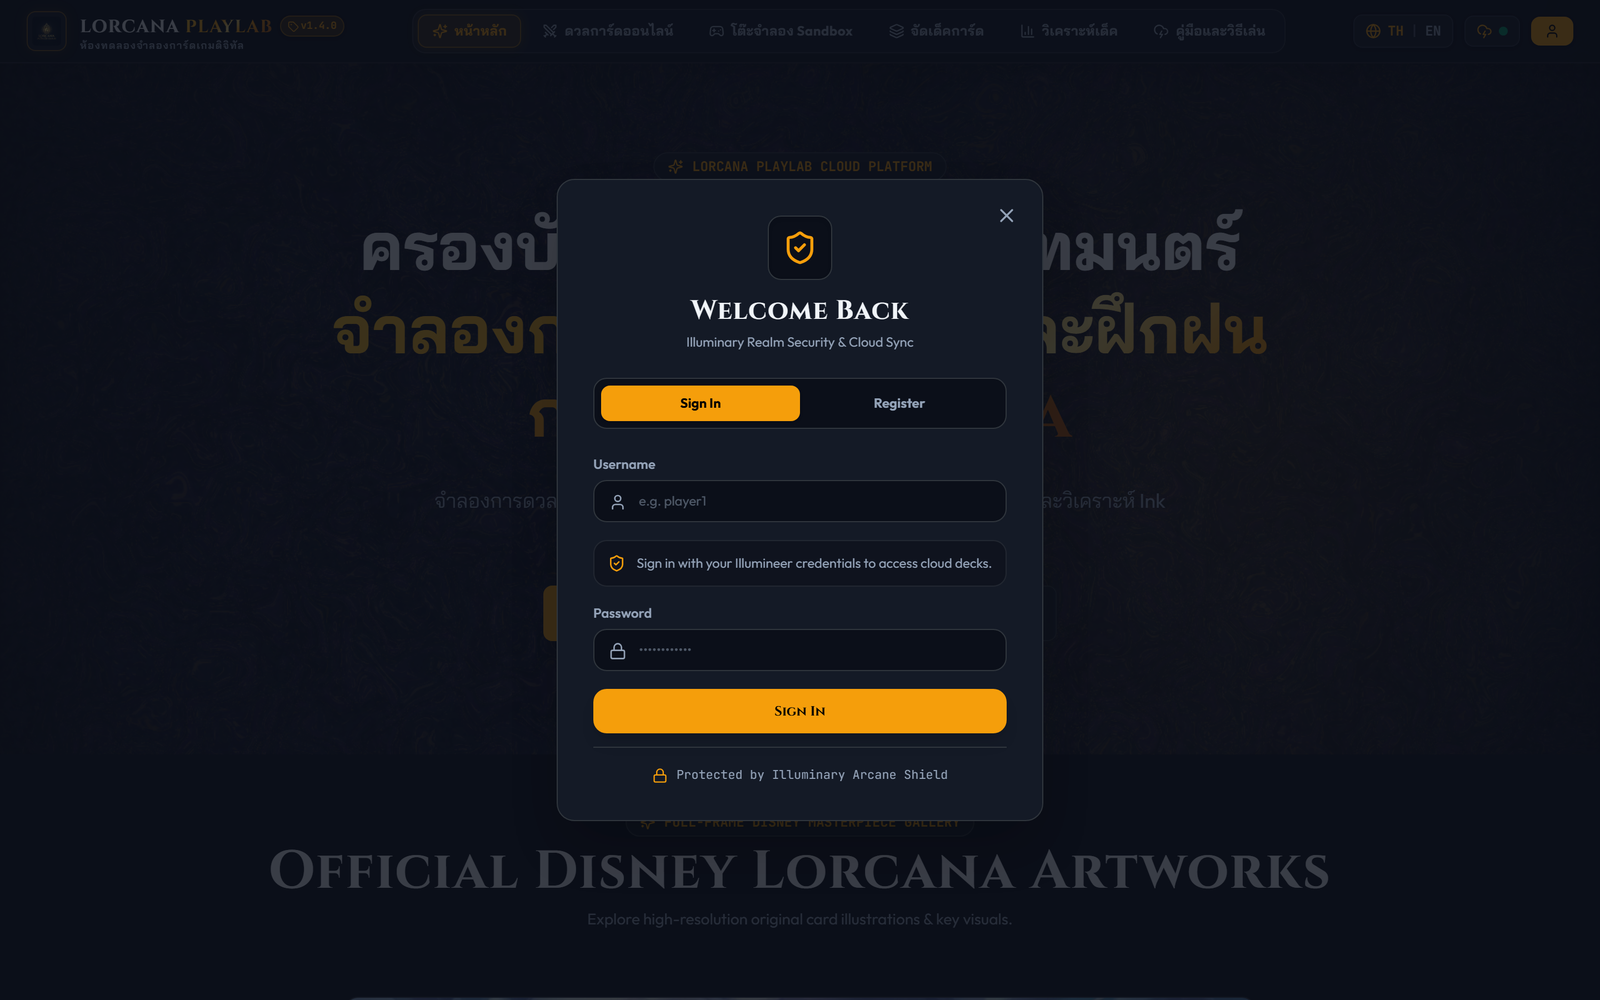
\includegraphics[width=\textwidth]{images/02_login_modal.png}
    \caption{หน้าต่าง Modal เข้าสู่ระบบ (Test User: io5)}
\end{subfigure}
\\[0.3cm]
\begin{subfigure}[b]{0.48\textwidth}
    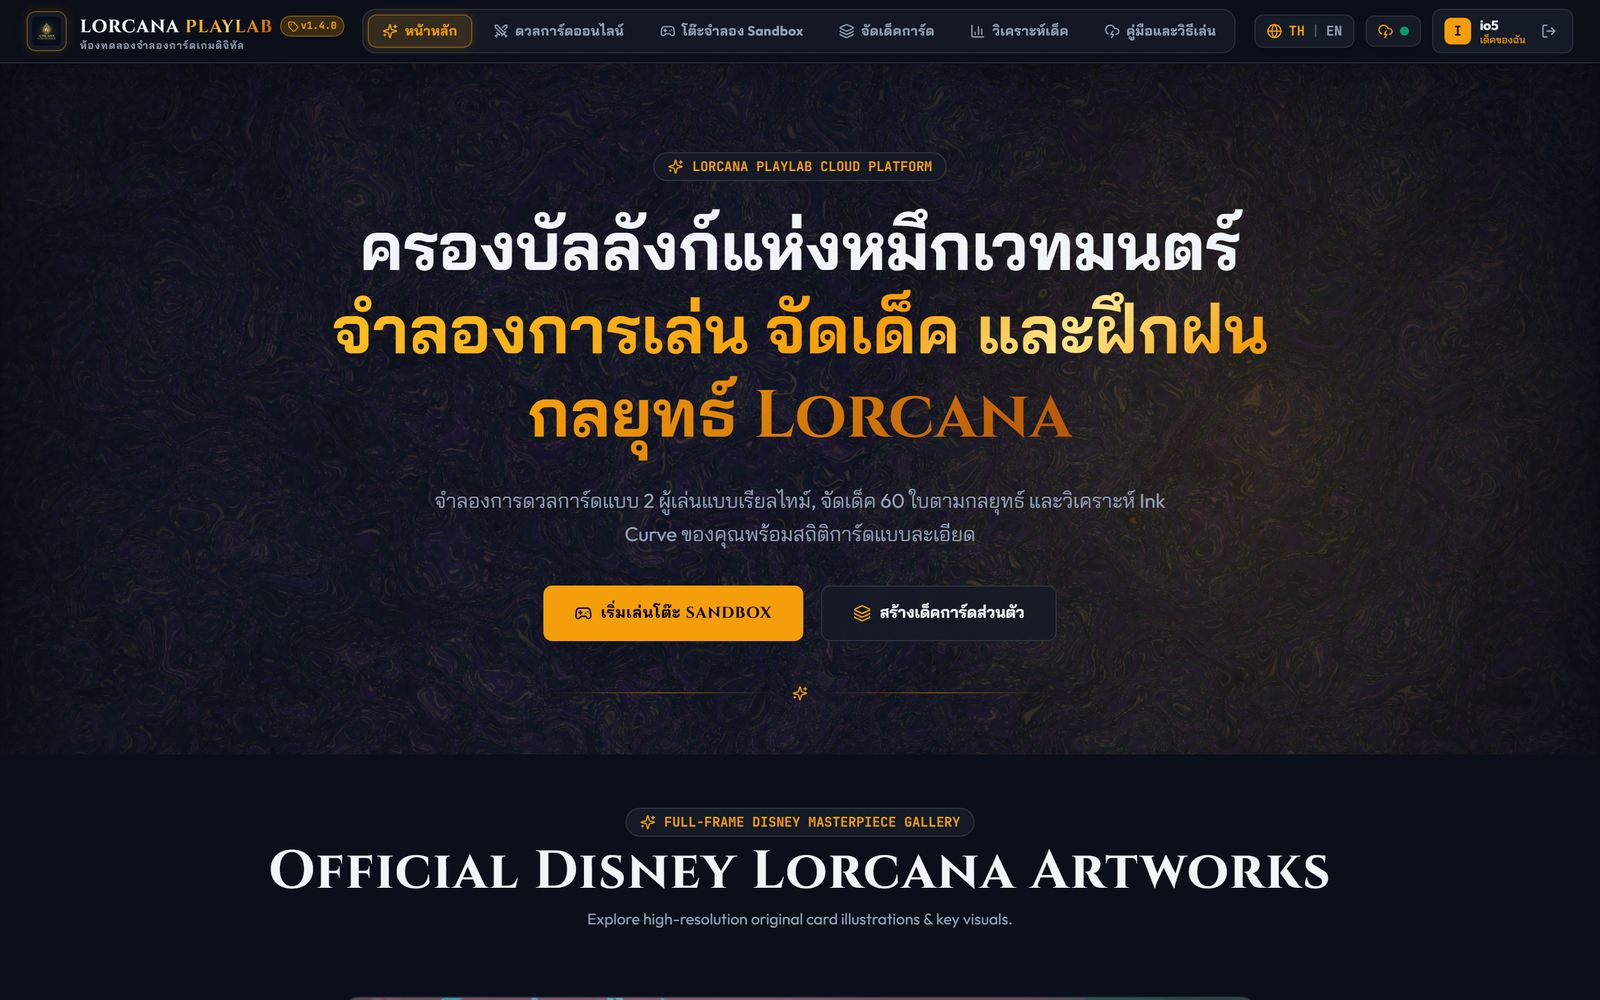
\includegraphics[width=\textwidth]{images/03_after_login_match_lobby.png}
    \caption{หน้า Match Lobby หลังเข้าสู่ระบบ}
\end{subfigure}
\hfill
\begin{subfigure}[b]{0.48\textwidth}
    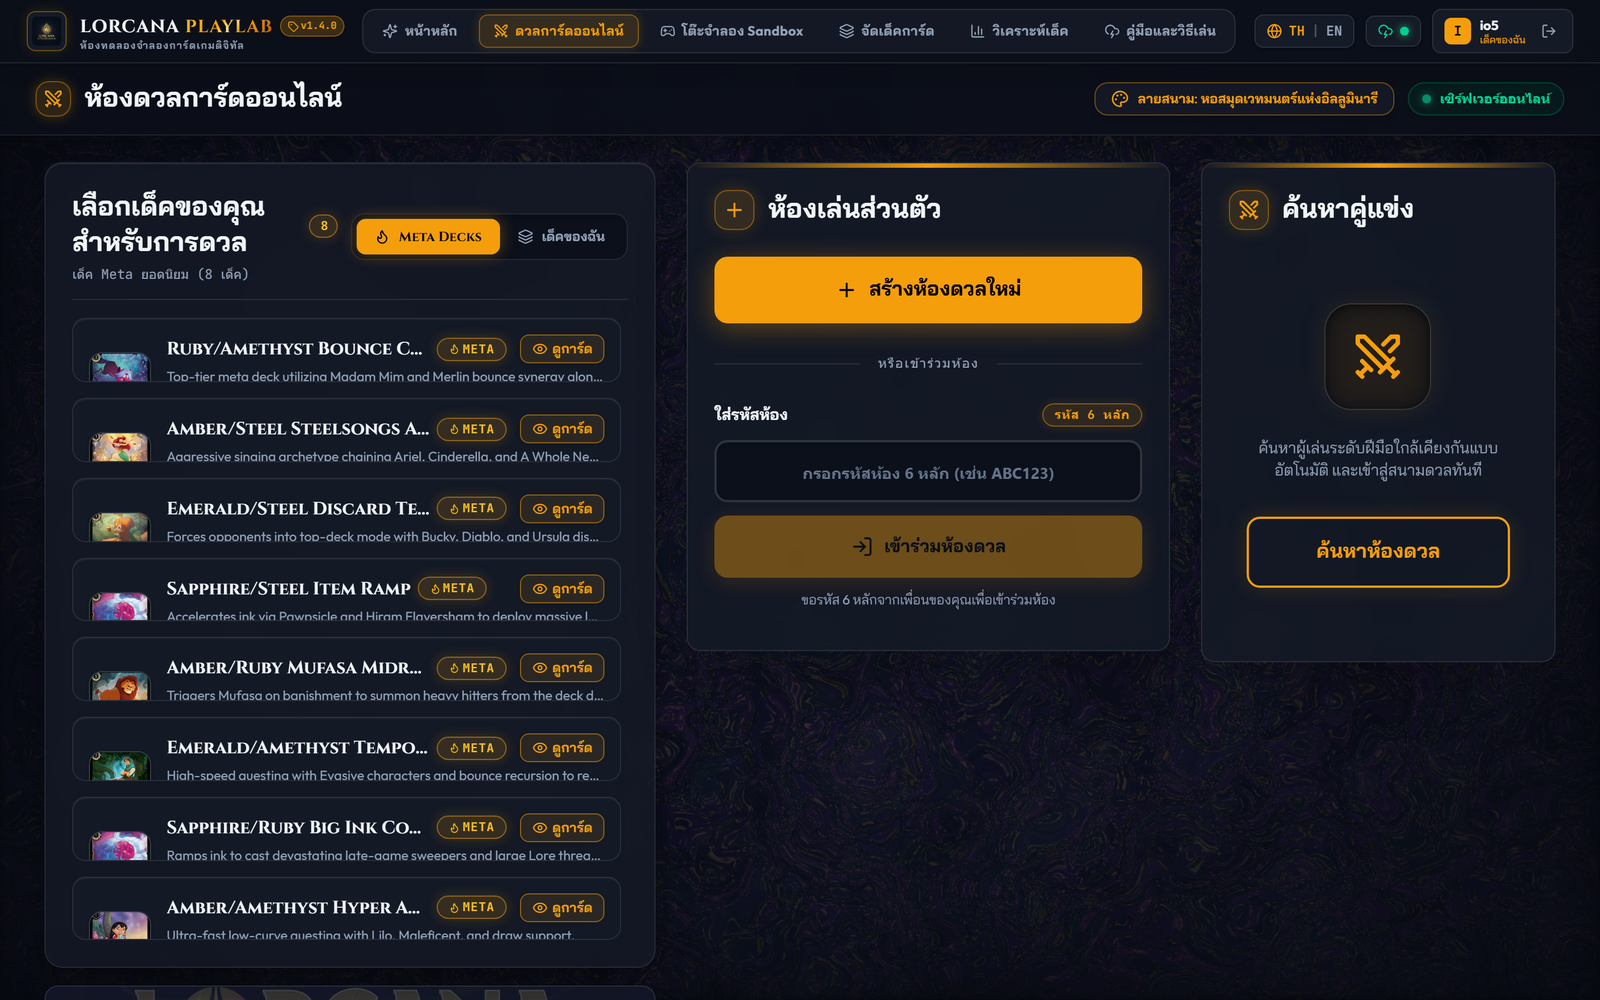
\includegraphics[width=\textwidth]{images/06_match_deck_select_room_modal.png}
    \caption{หน้าเลือกเด็ค สร้างรหัสห้อง และ Ranked Match}
\end{subfigure}
\caption{ภาพหน้าจอส่วนติดต่อผู้ใช้ระบบ Disney Lorcana PlayLab Cloud (ส่วนที่ 1)}
\label{fig:ui_gallery_1}
\end{figure}

\begin{figure}[H]
\centering
\begin{subfigure}[b]{0.48\textwidth}
    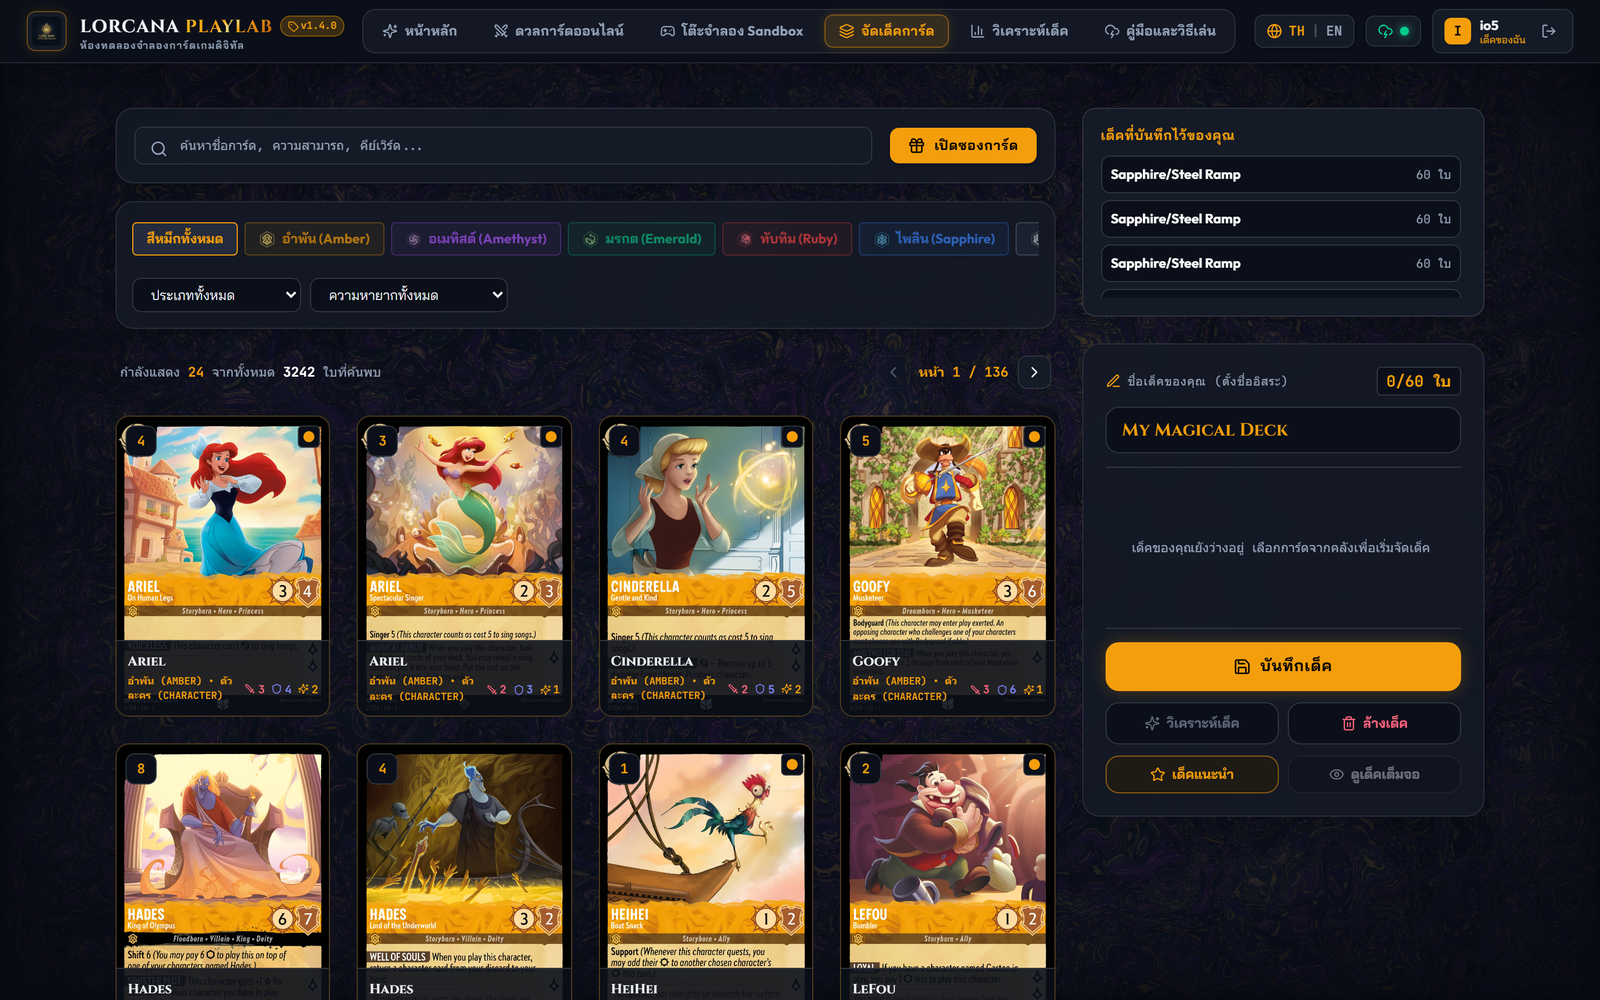
\includegraphics[width=\textwidth]{images/04_deck_builder.png}
    \caption{หน้าจัดการเด็คการ์ด (Deck Builder)}
\end{subfigure}
\hfill
\begin{subfigure}[b]{0.48\textwidth}
    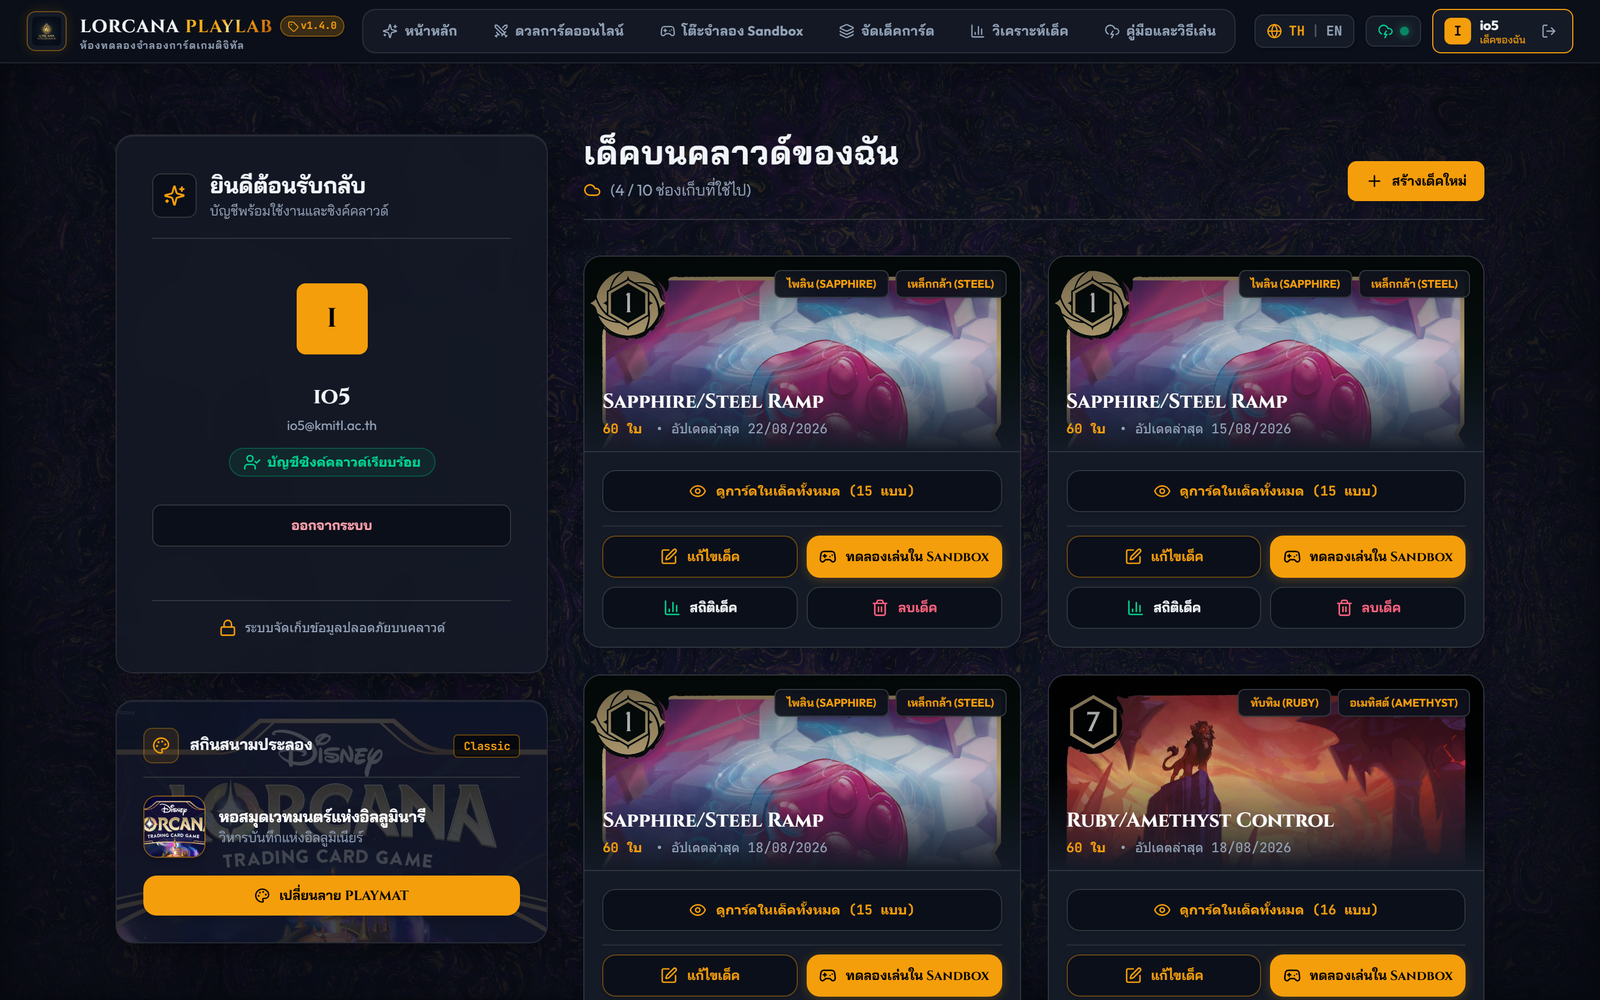
\includegraphics[width=\textwidth]{images/05_account_dashboard.png}
    \caption{หน้าข้อมูลบัญชีผู้ใช้และประวัติการเล่น (Account)}
\end{subfigure}
\\[0.3cm]
\begin{subfigure}[b]{0.48\textwidth}
    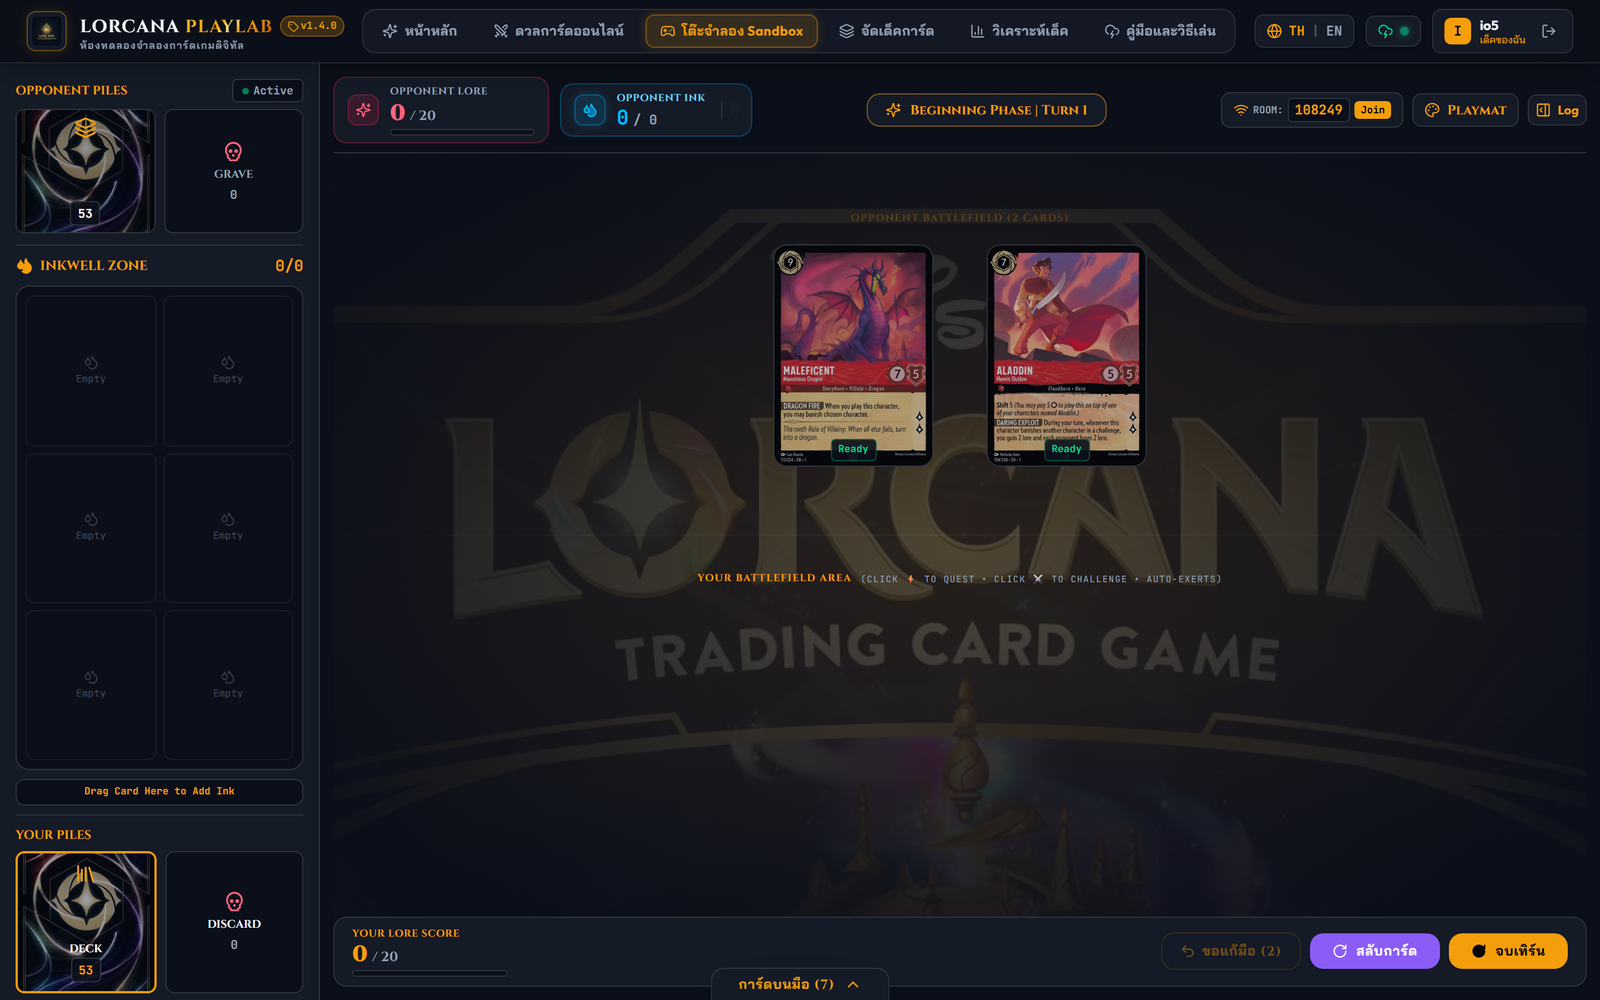
\includegraphics[width=\textwidth]{images/07_realtime_room_play.png}
    \caption{กระดานจำลองการเล่นการ์ดแบบเรียลไทม์ (Lorcana Board)}
\end{subfigure}
\hfill
\begin{subfigure}[b]{0.48\textwidth}
    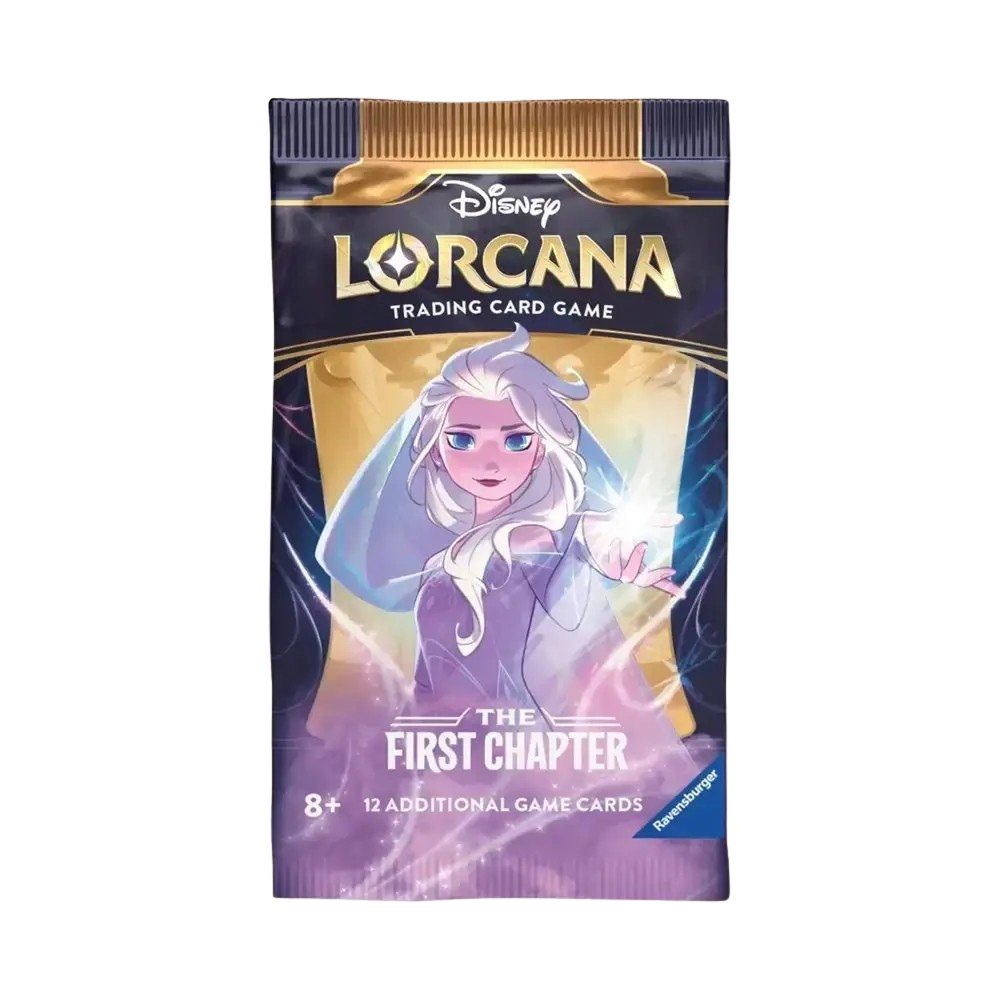
\includegraphics[width=\textwidth]{images/CardGachaDisney.png}
    \caption{ระบบจำลองการเปิดซองการ์ด 3D (Booster Pack)}
\end{subfigure}
\caption{ภาพหน้าจอส่วนติดต่อผู้ใช้ระบบ Disney Lorcana PlayLab Cloud (ส่วนที่ 2)}
\label{fig:ui_gallery_2}
\end{figure}

\begin{figure}[H]
\centering
\begin{subfigure}[b]{0.48\textwidth}
    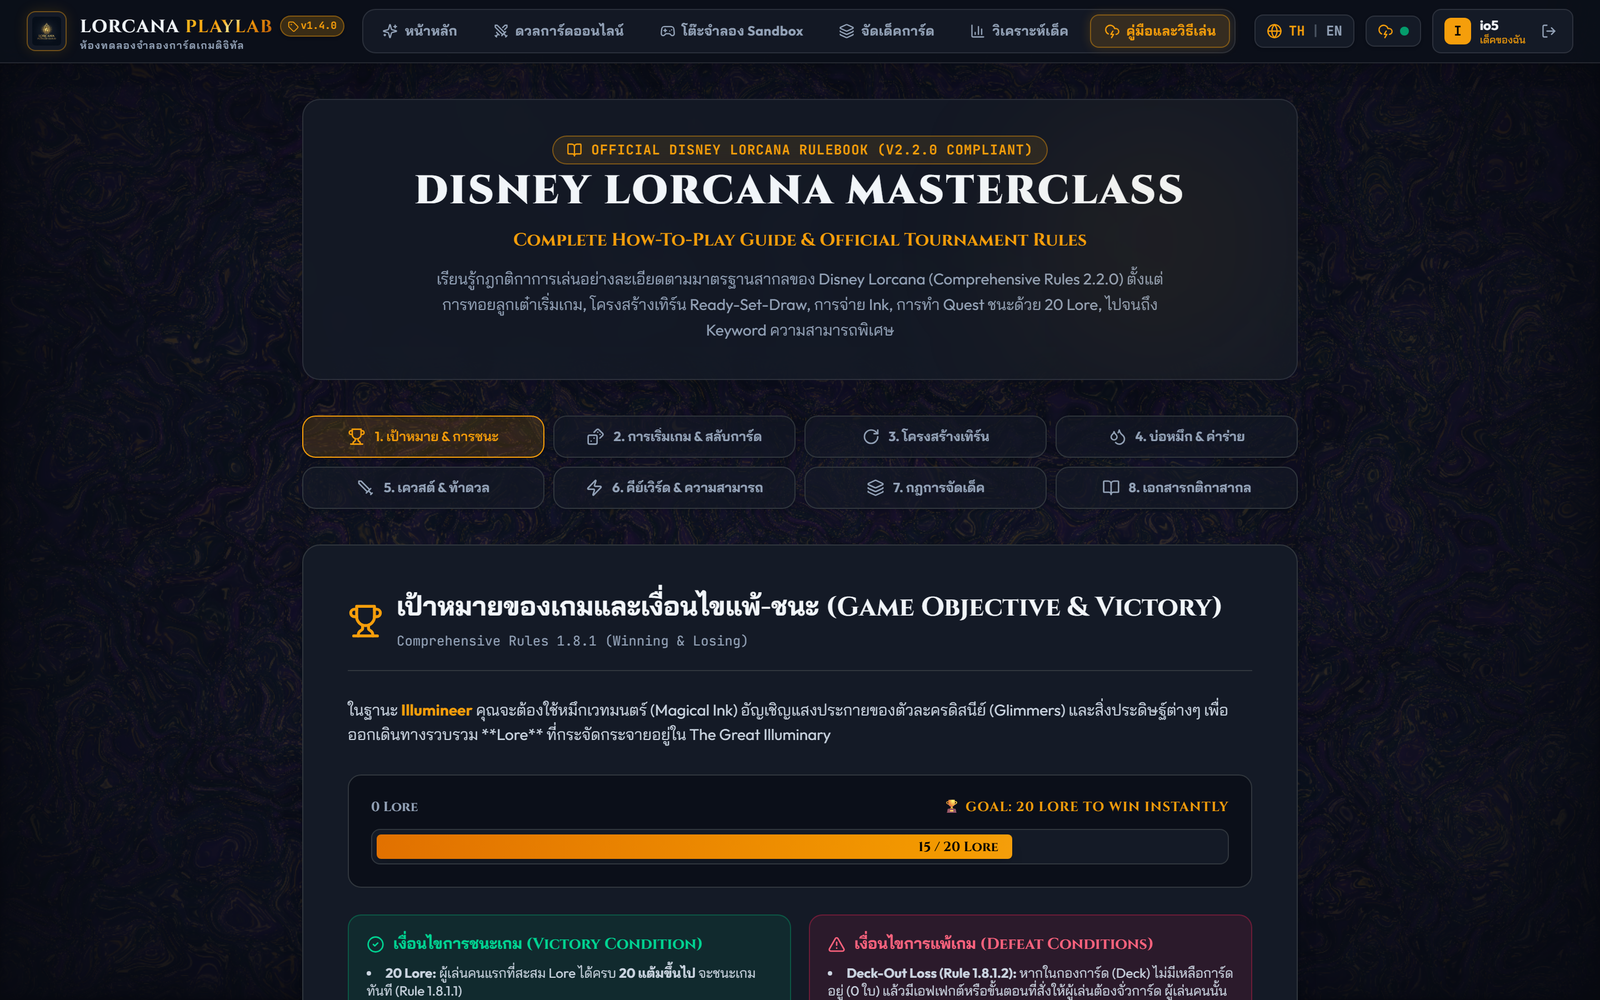
\includegraphics[width=\textwidth]{images/09_rules_guide.png}
    \caption{หน้ารวบรวมคู่มือและกฎกติกาการเล่น (Rules Guide)}
\end{subfigure}
\hfill
\begin{subfigure}[b]{0.48\textwidth}
    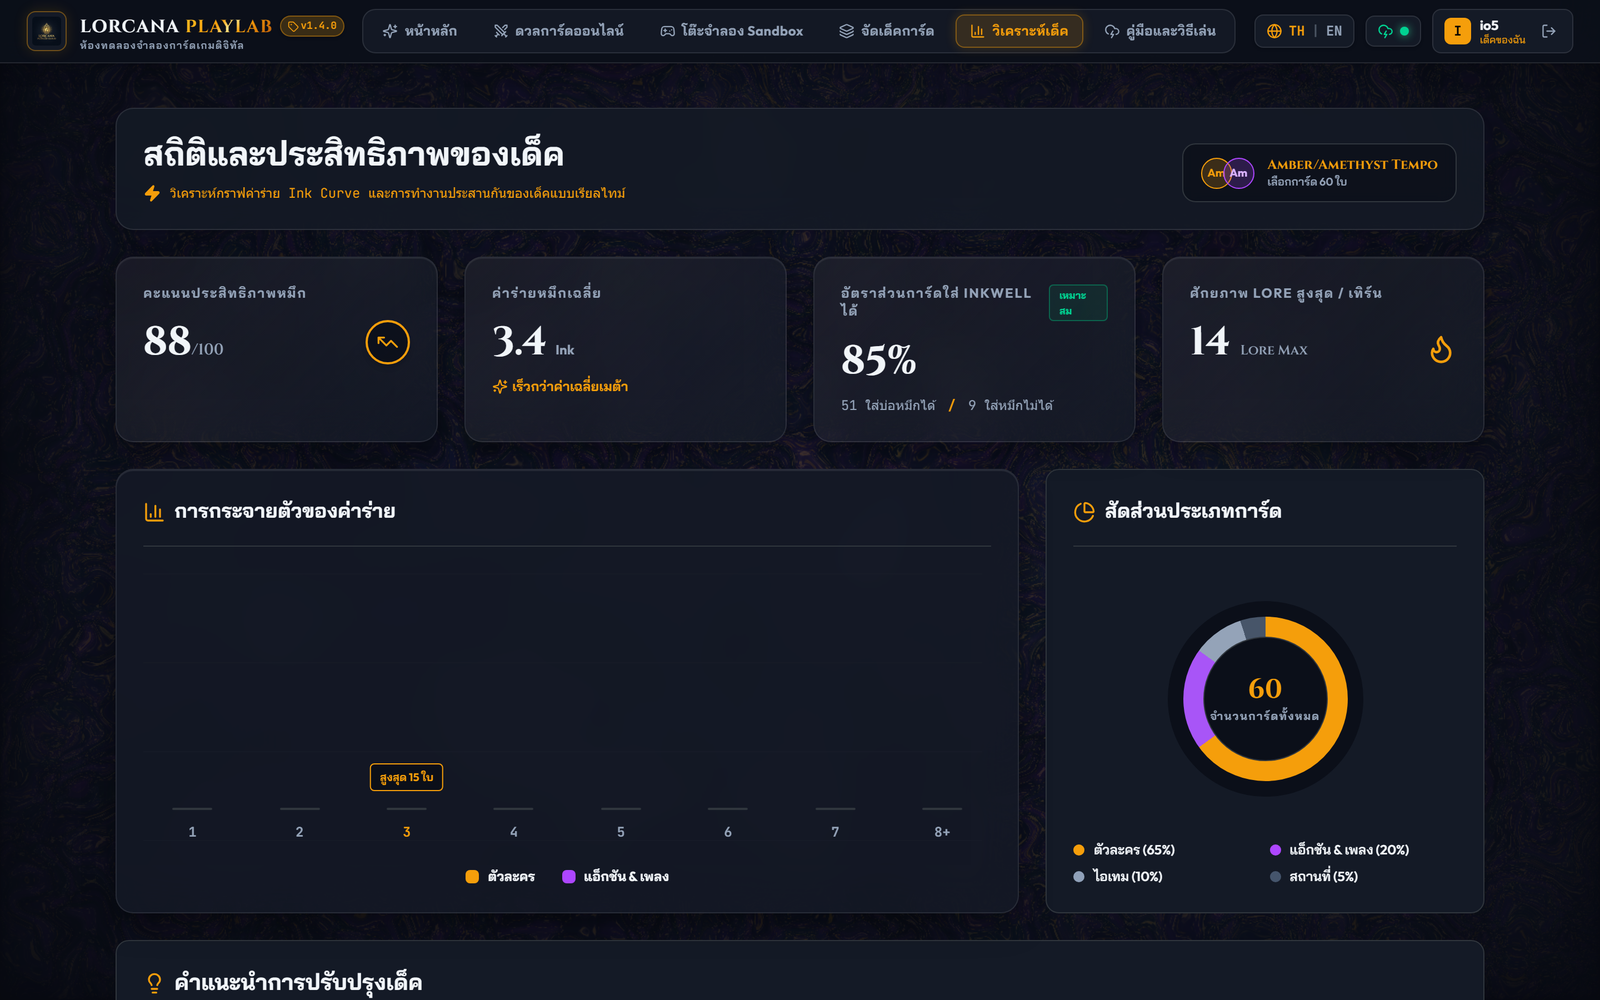
\includegraphics[width=\textwidth]{images/10_analytics_dashboard.png}
    \caption{หน้ารายงานสถิติและวิเคราะห์สมดุลเด็ค (Analytics)}
\end{subfigure}
\caption{ภาพหน้าจอหน้าระบบคู่มือการเล่นและระบบวิเคราะห์สถิติเด็ค}
\label{fig:ui_gallery_3}
\end{figure}

องค์ประกอบสำคัญของหน้าจอ Playmat ประกอบด้วย:
\begin{itemize}
    \item \textbf{Play Area (Battlefield):} พื้นที่ลงการ์ดตัวละคร ไอเทม และสถานที่ รองรับการลากวาง (Drag-and-Drop) อย่างอิสระ
    \item \textbf{Inkwell Tray:} พื้นที่คว่ำการ์ดเพื่อใช้เป็นหมึกค่าร่าย พร้อมตัวเลขแสดงจำนวน Unexerted / Total Ink
    \item \textbf{Lore Counter:} มาตรวัดแต้มความรู้ขนาดใหญ่ (0-20 แต้ม) พร้อมปุ่มปรับคะแนนและเอฟเฟกต์แอนิเมชัน
    \item \textbf{Card State Rotator:} กลไกการหมุนการ์ดแนวตั้ง (Ready) และแนวนอน 90 องศา (Exerted) เพื่อระบุว่าการ์ดถูกใช้งานแล้ว
    \item \textbf{3D Card Inspector \& Gacha:} ระบบเปิดซองการ์ด 3D สุ่มการ์ด 12 ใบพร้อมฟิสิกส์แอนิเมชันเปิดซอง
\end{itemize}

\section{รายละเอียดการพัฒนาส่วนประมวลผลบนคลาวด์ (AWS Microservices)}
ฟังก์ชัน Lambda ได้รับการพัฒนาด้วย TypeScript และคอมไพล์เป็น Node.js 20.x แบ่งเป็น 4 โมดูลหลัก:
\begin{enumerate}
    \item \textbf{\texttt{lorcana-auth}:} จัดการการสมัครสมาชิก (\texttt{register}) และการเข้าสู่ระบบ (\texttt{login}) โดยตรวจสอบความถูกต้องของรหัสผ่านด้วย bcrypt และออก JWT Token
    \item \textbf{\texttt{lorcana-deck}:} จัดการ CRUD เด็คการ์ดของผู้ใช้ โดยดึงข้อมูลจากตาราง DynamoDB \texttt{LorcanaDecks} ตาม \texttt{userId}
    \item \textbf{\texttt{lorcana-room-handler}:} จัดการการเชื่อมต่อ WebSocket จัดการ Action \texttt{JOIN\_ROOM}, \texttt{CARD\_MOVED}, \texttt{CARD\_EXERTED}, \texttt{INK\_PLAYED}, \texttt{LORE\_UPDATED}, \texttt{TURN\_PASSED} และ Broadcast ไปยังผู้เล่นคู่แข่งผ่าน \texttt{ApiGatewayManagementApiClient}
    \item \textbf{\texttt{lorcana-analyzer}:} รับงานวิเคราะห์เด็คการ์ดจากคิว Amazon SQS และประมวลผลค่าสถิติ Ink Curve แบบ Asynchronous
\end{enumerate}

\section{แผนและผลการทดสอบคุณภาพระบบ (Quality Assurance \& Test Verification)}
การทดสอบคุณภาพระบบดำเนินตามรูปแบบพีระมิดการทดสอบ (Testing Pyramid) ครอบคลุม Unit Test, Integration Test, End-to-End Test และ Security Test ดังแสดงในตารางที่ \ref{tab:qa_results}:

\begin{table}[H]
\centering
\caption{ผลการทดสอบคุณภาพระบบโดยรวม (Master QA Test Matrix)}
\label{tab:qa_results}
\small
\begin{tabularx}{\textwidth}{p{1.4cm}p{2.2cm}Xp{1.5cm}p{1.5cm}}
\toprule
\textbf{Test ID} & \textbf{ระดับการทดสอบ} & \textbf{เงื่อนไขและกรณีทดสอบ} & \textbf{Latency} & \textbf{ผลการทดสอบ} \\
\midrule
TC-AUTH-01 & Integration & สมัครสมาชิกใหม่ (POST /auth/register) & 180ms & ผ่าน (201 Created) \\
TC-AUTH-02 & Integration & เข้าสู่ระบบด้วยรหัสผ่านถูกต้อง (POST /auth/login) & 145ms & ผ่าน (200 + JWT) \\
TC-AUTH-03 & Security & เข้าสู่ระบบด้วยรหัสผ่านผิด & 120ms & ผ่าน (401 Unauthorized) \\
TC-DECK-01 & Integration & บันทึกเด็คใหม่ 60 ใบ (POST /decks) & 95ms & ผ่าน (201 Created) \\
TC-DECK-02 & Integration & ดึงรายการเด็คของผู้ใช้ (GET /decks) & 68ms & ผ่าน (200 OK) \\
TC-DECK-03 & Integration & ลบเด็คการ์ด (DELETE /decks/\{id\}) & 72ms & ผ่าน (200 OK) \\
TC-WS-01 & E2E & เชื่อมต่อ WSS Persistent Socket (\$connect) & 45ms & ผ่าน (101 Connected) \\
TC-WS-02 & E2E Multi-User & ผู้เล่น 2 คนเข้าห้องเดียวกัน (JOIN\_ROOM) & 82ms & ผ่าน (Room Paired) \\
TC-WS-03 & E2E Multi-User & ซิงค์การลากวางการ์ด (CARD\_MOVED) & 64ms & ผ่าน (<100ms Target) \\
TC-WS-04 & E2E Multi-User & ซิงค์การหมุนการ์ด (CARD\_EXERTED) & 58ms & ผ่าน (<100ms Target) \\
TC-WS-05 & E2E Multi-User & ซิงค์แต้ม Lore (LORE\_UPDATED) & 52ms & ผ่าน (<100ms Target) \\
TC-WS-06 & Fault Tolerance & จำลองเน็ตหลุดและกู้คืน (Auto-Reconnect) & 310ms & ผ่าน (State Restored) \\
TC-SEC-01 & Security (OWASP) & ตรวจสอบการเข้ารหัสรหัสผ่านใน DynamoDB & - & ผ่าน (bcrypt 10 rounds) \\
TC-SEC-02 & Security (OWASP) & ป้องกัน Injection ใน WebSocket Action Payload & - & ผ่าน (Schema Validated) \\
\bottomrule
\end{tabularx}
\end{table}

ผลการทดสอบยืนยันว่าการซิงค์ข้อมูลกระดานผ่าน AWS API Gateway WebSockets มีความหน่วงเฉลี่ยระหว่าง \textbf{52--82 มิลลิวินาที} ซึ่งผ่านเกณฑ์เป้าหมาย Sub-100ms ได้อย่างสมบูรณ์

% =============================================================
% CHAPTER 5
% =============================================================
\chapter{สรุปผลการดำเนินงานและแผนงานในอนาคต (Conclusions \& Future Roadmap)}

\section{สรุปผลการดำเนินงานความก้าวหน้า Stage 2}
การดำเนินงานโครงงาน \textbf{Disney Lorcana PlayLab Cloud} ในระยะที่ 2 (Stage 2) ครอบคลุมการพัฒนาตามแผนงาน Sprint 1 ถึง Sprint 3 สำเร็จลุล่วง 100\% ตามข้อกำหนดของรายวิชา Cloud Technology โดยมีผลสัมฤทธิ์สำคัญดังนี้:
\begin{enumerate}
    \item พัฒนาส่วนติดต่อผู้ใช้จำลองกระดานเล่นการ์ด Disney Lorcana ที่สมบูรณ์แบบ รองรับกฎการเล่นมาตรฐาน ฐานข้อมูลการ์ดทางการกว่า 3,200 ใบ และระบบ 3D Card Inspector
    \item ออกแบบและปรับใช้สถาปัตยกรรมคลาวด์แบบไร้เซิร์ฟเวอร์เต็มรูปแบบ (100\% Serverless) บน AWS ประกอบด้วย AWS Lambda, Amazon DynamoDB, และ AWS API Gateway (HTTP \& WebSocket)
    \item บรรลุเป้าหมายความเร็วในการซิงค์ข้อมูลระหว่างผู้เล่นด้วยความหน่วงต่ำกว่า 100 มิลลิวินาที (เฉลี่ย 52--82ms)
    \item เอาชนะข้อจำกัดสิทธิ์บน AWS Academy Learner Lab ได้อย่างมีประสิทธิภาพผ่านการใช้ Pre-provisioned LabRole และสคริปต์ Deployment อัตโนมัติ
    \item ควบคุมค่าใช้จ่ายโครงสร้างพื้นฐานทั้งหมดให้อยู่ในโควตา AWS Free Tier (0.00 ดอลลาร์สหรัฐ) สอดคล้องกับกรอบงบประมาณที่กำหนด
\end{enumerate}

\section{แผนงานการพัฒนาสำหรับ Stage 3 (Sprint 4 ถึง Sprint 7)}
\begin{enumerate}
    \item \textbf{Sprint 4 (Async Deck Analyzer via Amazon SQS):} พัฒนาระบบประมวลผลวิเคราะห์เด็คการ์ดเชิงลึก คำนวณความเสี่ยง ค่าร่ายเฉลี่ย และแนะนำการปรับเด็คโดยใช้ Amazon SQS รับงานและส่งต่อให้ Lambda ทำงานเบื้องหลัง
    \item \textbf{Sprint 5 (Observability, Monitoring \& Security Hardening):} สร้าง Amazon CloudWatch Dashboard แสดงผลแบบรวมศูนย์ และตั้งค่า CloudWatch Alarms แจ้งเตือนเมื่อเกิด Error Rate สูงกว่า 1\%
    \item \textbf{Sprint 6 (Load Testing \& High Concurrency Simulation):} ดำเนินการทดสอบโหลดด้วยเครื่องมือ Artillery เพื่อจำลองผู้เล่นพร้อมกัน 100--500 ผู้ใช้ และทดสอบความทนทานของระบบ WebSocket Auto-reconnection
    \item \textbf{Sprint 7 (Final Report \& Video Presentation):} จัดทำรายงานฉบับสมบูรณ์ วิดีโอสาธิตการใช้งานระบบ และเตรียมการนำเสนอโครงงานในรอบสุดท้าย
\end{enumerate}

\section{บทเรียนที่ได้รับและการปรับปรุงกระบวนการทำงาน (Retrospective)}
\begin{enumerate}
    \item \textbf{ความสำคัญของการออกแบบ Interface และ Contract First:} การกำหนดรูปแบบ JSON Payload ของ WebSocket และ DynamoDB Schema ล่วงหน้าช่วยลดข้อผิดพลาดในการรวมระบบระหว่าง Frontend และ Cloud Backend ได้อย่างมาก
    \item \textbf{การเข้าใจสภาพแวดล้อมคลาวด์แบบจำกัดสิทธิ์:} การเตรียมแผนสำรองสำหรับข้อจำกัดด้าน IAM Role บน AWS Learner Lab ทำให้ทีมงานสามารถส่งมอบงานได้ตรงตามกำหนดการโดยไม่เกิดความล่าช้า
    \item \textbf{การบริหารจัดการสถาปัตยกรรมไร้เซิร์ฟเวอร์:} การเลือกใช้บริการ Serverless ช่วยลดภาระงานด้านการดูแลระบบลงได้อย่างมหาศาล ทำให้ทีมงานสามารถมุ่งเน้นการพัฒนาฟีเจอร์และปรับปรุงประสบการณ์ของผู้ใช้งานได้อย่างเต็มที่
\end{enumerate}

% -------------------------------------------------------------
% REFERENCES (บรรณานุกรม)
% -------------------------------------------------------------
\chapter*{บรรณานุกรม (References)}
\addcontentsline{toc}{chapter}{บรรณานุกรม (References)}

\noindent [1] Ravensburger \& Disney. (2023). \textit{Disney Lorcana Trading Card Game Official Rules and Card Database}. [Online]. Available: \url{https://www.disneylorcana.com}\\[0.3cm]
\noindent [2] Amazon Web Services. (2026). \textit{AWS Lambda Developer Guide: Building Event-Driven Serverless Applications}. [Online]. Available: \url{https://docs.aws.amazon.com/lambda/}\\[0.3cm]
\noindent [3] Amazon Web Services. (2026). \textit{Amazon API Gateway Developer Guide: About WebSocket APIs in API Gateway}. [Online]. Available: \url{https://docs.aws.amazon.com/apigateway/latest/developerguide/apigateway-websocket-api.html}\\[0.3cm]
\noindent [4] Amazon Web Services. (2026). \textit{Amazon DynamoDB Developer Guide: Core Components and Best Practices for NoSQL Design}. [Online]. Available: \url{https://docs.aws.amazon.com/amazondynamodb/}\\[0.3cm]
\noindent [5] Amazon Web Services. (2026). \textit{AWS Well-Architected Framework: Reliability, Security, and Cost Optimization Pillars}. [Online]. Available: \url{https://aws.amazon.com/architecture/well-architected/}\\[0.3cm]
\noindent [6] React Working Group. (2026). \textit{React 19 Documentation: Concurrent Features and Server Components}. [Online]. Available: \url{https://react.dev}\\[0.3cm]
\noindent [7] Tailwind Labs. (2026). \textit{Tailwind CSS v4.0 Alpha/Release Documentation}. [Online]. Available: \url{https://tailwindcss.com}\\[0.3cm]
\noindent [8] Framer. (2026). \textit{Framer Motion: Production-Ready Animation Library for React}. [Online]. Available: \url{https://www.framer.com/motion/}\\[0.3cm]
\noindent [9] IETF (Internet Engineering Task Force). (2011). \textit{RFC 6455: The WebSocket Protocol}. [Online]. Available: \url{https://tools.ietf.org/html/rfc6455}

% -------------------------------------------------------------
% APPENDIX (ภาคผนวก)
% -------------------------------------------------------------
\chapter*{ภาคผนวก (Appendix)}
\addcontentsline{toc}{chapter}{ภาคผนวก (Appendix)}

\section*{ตัวอย่างโค้ดสคริปต์ Deployment บน AWS Learner Lab (\texttt{scripts/deploy\_ws.sh})}

\begin{lstlisting}[language=bash, caption={สคริปต์ Deploy WebSocket Lambda \& API Gateway บน AWS Learner Lab}]
#!/bin/bash
# scripts/deploy_ws.sh - Deploy Real-Time WebSocket Infrastructure
set -e

echo "=== 1. Building Backend TypeScript ==="
cd ../backend
npm install
npx tsc --outDir dist

echo "=== 2. Packaging Lambda Handler ==="
cd dist/room
zip -r ../../../room-handler.zip .
cd ../../..

echo "=== 3. Updating Lambda Code via AWS CLI ==="
aws lambda update-function-code \
    --function-name lorcana-room-handler \
    --zip-file fileb://room-handler.zip \
    --region us-east-1

echo "=== 4. Verifying WebSocket API Gateway Integration ==="
API_ID=$(aws apigatewayv2 get-apis --query "Items[?Name=='lorcana-ws-api'].ApiId" --output text)
echo "WebSocket API ID: $API_ID"
echo "WebSocket Endpoint: wss://${API_ID}.execute-api.us-east-1.amazonaws.com/prod"

echo "=== Deployment Completed Successfully ==="
\end{lstlisting}

\end{document}
